\documentclass[11pt,a4paper]{article}

\usepackage[margin=2.5cm]{geometry}
\usepackage{amsmath,amssymb,amsthm}
\usepackage{graphicx}
\usepackage{booktabs}
\usepackage{caption}
\usepackage{subcaption}
\usepackage{hyperref}
\usepackage{xcolor}
\usepackage{float}
\usepackage{enumitem}

\hypersetup{colorlinks=true, linkcolor=blue!60!black, citecolor=blue!60!black, urlcolor=blue!60!black}

\newtheorem{definition}{Definition}
\newtheorem{remark}{Remark}

\title{\textbf{Simulation Experiments for Meta-MAPG Dissertation}\\[0.5em]
\large Gradient Term Decomposition, Extended Game Suite, and N-Agent Scaling}
\author{Generated by Claude for Yevhen Shcherbinin}
\date{March 2026}

\begin{document}
\maketitle

\begin{abstract}
This report documents 15 simulation experiments validating the Meta-Multiagent Policy Gradient (Meta-MAPG) theorem of Kim et al.\ (2021) in stateless matrix games. The core contribution is the \textbf{gradient term decomposition}: measuring the separate magnitudes of Terms 1 (direct), 2 (own-learning), and 3 (peer-learning) across five game types, showing how game structure determines which terms drive convergence. We extend the analysis to N-agent games (3, 5, 7 players), stochastic gradient estimation, hyperparameter sensitivity, and formal convergence rate quantification. All experiments use exact analytic gradients from matrix game payoff structures with NumPy; no ML frameworks are involved.
\end{abstract}

\tableofcontents
\newpage

% ══════════════════════════════════════════════════════════════════════
\section{Background and Setup}
% ══════════════════════════════════════════════════════════════════════

\subsection{The Meta-MAPG Three-Term Gradient}

The Meta-MAPG theorem decomposes the policy gradient for agent $i$ in a multi-agent stochastic game into three terms:
\begin{equation}
\nabla_{\phi^i_0} V^i = \underbrace{\nabla_{\phi^i} V^i\big|_{\phi_0}}_{\text{Term 1: direct}} + \underbrace{\nabla_{\phi^i} V^i\big|_{\phi_K} \cdot (J_{ii} - I)}_{\text{Term 2: own-learning}} + \underbrace{\sum_{j \neq i} \nabla_{\phi^j} V^i\big|_{\phi_K} \cdot J_{ji}}_{\text{Term 3: peer-learning}}
\label{eq:meta-mapg}
\end{equation}
where $J_{ji} = \partial \phi^j_K / \partial \phi^i_0$ is the Jacobian tracking how agent $i$'s initial parameters affect agent $j$'s parameters after $K$ inner-loop steps. The four methods compared are:

\begin{center}
\begin{tabular}{llll}
\toprule
\textbf{Method} & \textbf{Terms Used} & \textbf{Awareness} & \textbf{Source} \\
\midrule
Independent PG & Term 1 only & None & Baseline \\
LOLA & Terms 1 + 3 (approx.) & Peer learning & Foerster et al.\ (2018) \\
Meta-PG & Terms 1 + 2 & Own learning & Al-Shedivat et al.\ (2018) \\
Meta-MAPG & Terms 1 + 2 + 3 & Full & Kim et al.\ (2021) \\
\bottomrule
\end{tabular}
\end{center}

\subsection{Game Environments}

All games are two-player stateless (matrix) games. Agent $i$ plays action $a^i \in \{0, 1\}$ with probability $\pi^i(a^i = 0) = \sigma(\phi^i)$, where $\sigma$ is the sigmoid function.

\begin{center}
\begin{tabular}{lccl}
\toprule
\textbf{Game} & $R^1$ & $R^2$ & \textbf{Nash (mixed)} \\
\midrule
Matching Pennies & $\begin{psmallmatrix} 1 & -1 \\ -1 & 1 \end{psmallmatrix}$ & $-R^1$ & $(0.5, 0.5)$ \\[0.8em]
Prisoner's Dilemma & $\begin{psmallmatrix} 3 & 0 \\ 4 & 1 \end{psmallmatrix}$ & $\begin{psmallmatrix} 3 & 4 \\ 0 & 1 \end{psmallmatrix}$ & Pure: $(D, D)$ \\[0.8em]
Stag Hunt & $\begin{psmallmatrix} 4 & 0 \\ 3 & 3 \end{psmallmatrix}$ & $\begin{psmallmatrix} 4 & 3 \\ 0 & 3 \end{psmallmatrix}$ & $(0.75, 0.75)$ \\[0.8em]
Chicken & $\begin{psmallmatrix} 0 & 4 \\ 1 & 2 \end{psmallmatrix}$ & $\begin{psmallmatrix} 0 & 1 \\ 4 & 2 \end{psmallmatrix}$ & $(0.67, 0.67)$ \\[0.8em]
Battle of the Sexes & $\begin{psmallmatrix} 3 & 0 \\ 0 & 1 \end{psmallmatrix}$ & $\begin{psmallmatrix} 1 & 0 \\ 0 & 3 \end{psmallmatrix}$ & $(0.75, 0.25)$ \\
\bottomrule
\end{tabular}
\end{center}

Additionally, we define N-agent games:
\begin{itemize}[nosep]
\item \textbf{N-Player Public Goods}: Agent cooperates (cost $c$) or free-rides; total contributions multiplied by $m/N$ and shared equally.
\item \textbf{N-Player Stag Hunt}: Cooperation succeeds only if $\geq T$ agents cooperate (threshold variant).
\end{itemize}

\subsection{Implementation}

All gradients are computed analytically from the payoff matrices. For $V^i(\phi^1, \phi^2) = \sum_{a^1, a^2} \pi^1(a^1) \pi^2(a^2) R^i_{a^1, a^2}$, the exact policy gradient is:
\[
\frac{\partial V^i}{\partial \phi^j} = \frac{\partial V^i}{\partial p^j} \cdot \sigma'(\phi^j)
\]
Second derivatives (needed for LOLA and Jacobian tracking) use a mix of analytic cross-derivatives and finite differences ($\epsilon = 10^{-5}$) for self-second-derivatives. N-agent gradients use finite differences throughout.

\textbf{Software}: Python 3.14, NumPy, Matplotlib. No ML frameworks.

\newpage
% ══════════════════════════════════════════════════════════════════════
\section{Experiments 1--4: Baseline Results}
\label{sec:baseline}
% ══════════════════════════════════════════════════════════════════════

These reproduce the core demonstrations from the existing simulation code.

\subsection{Experiment 1: Matching Pennies}

\begin{figure}[H]
\centering
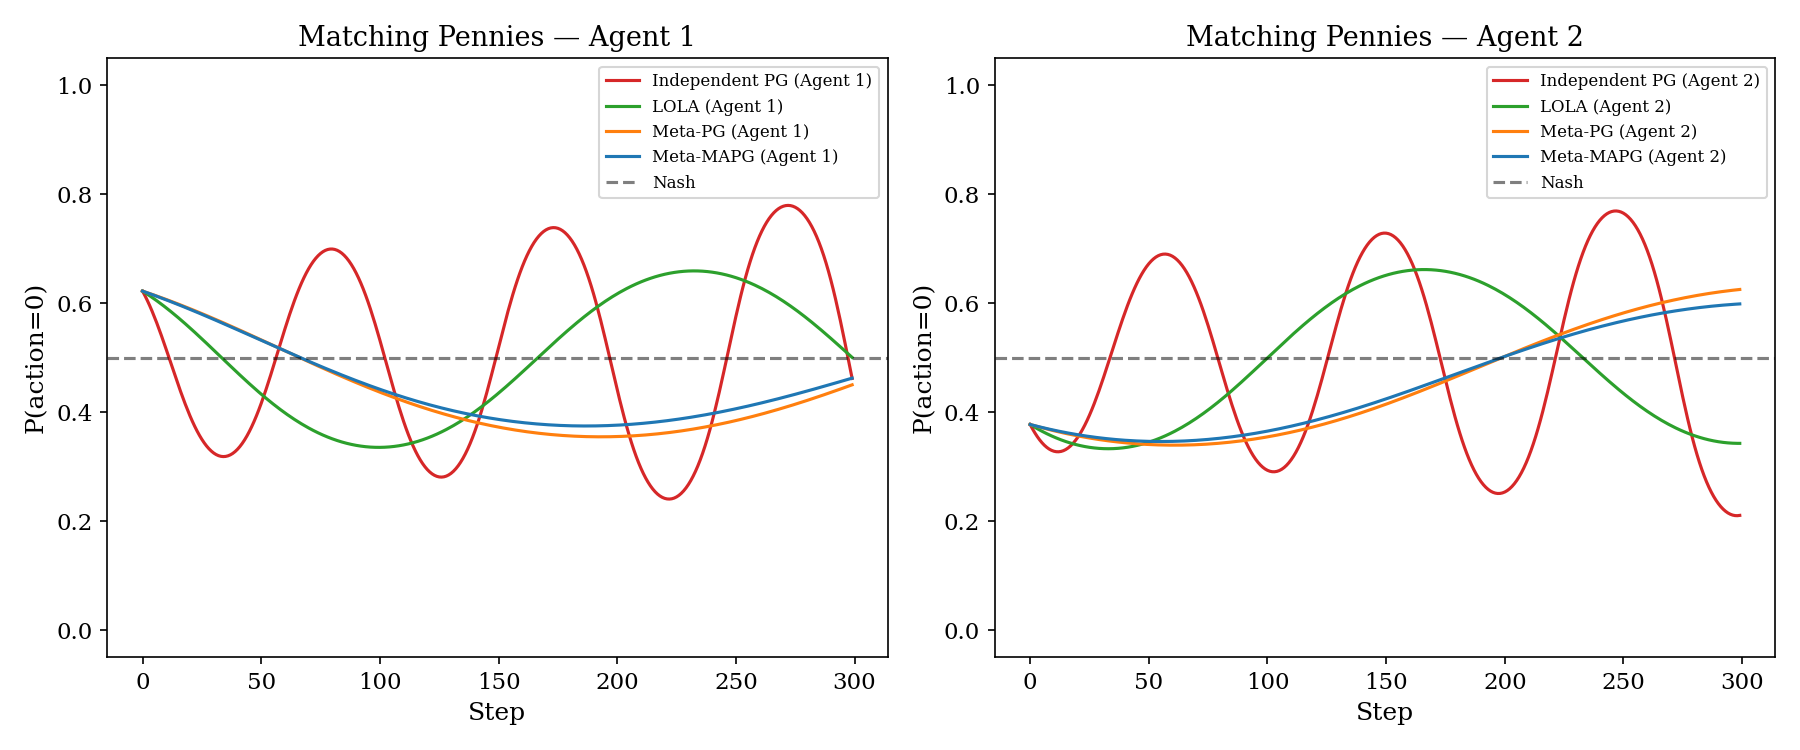
\includegraphics[width=\textwidth]{figures/matching_pennies_convergence.png}
\caption{Policy convergence in Matching Pennies. Meta-MAPG converges closest to Nash ($p = 0.5$). Independent PG oscillates and diverges.}
\label{fig:mp-convergence}
\end{figure}

\begin{figure}[H]
\centering
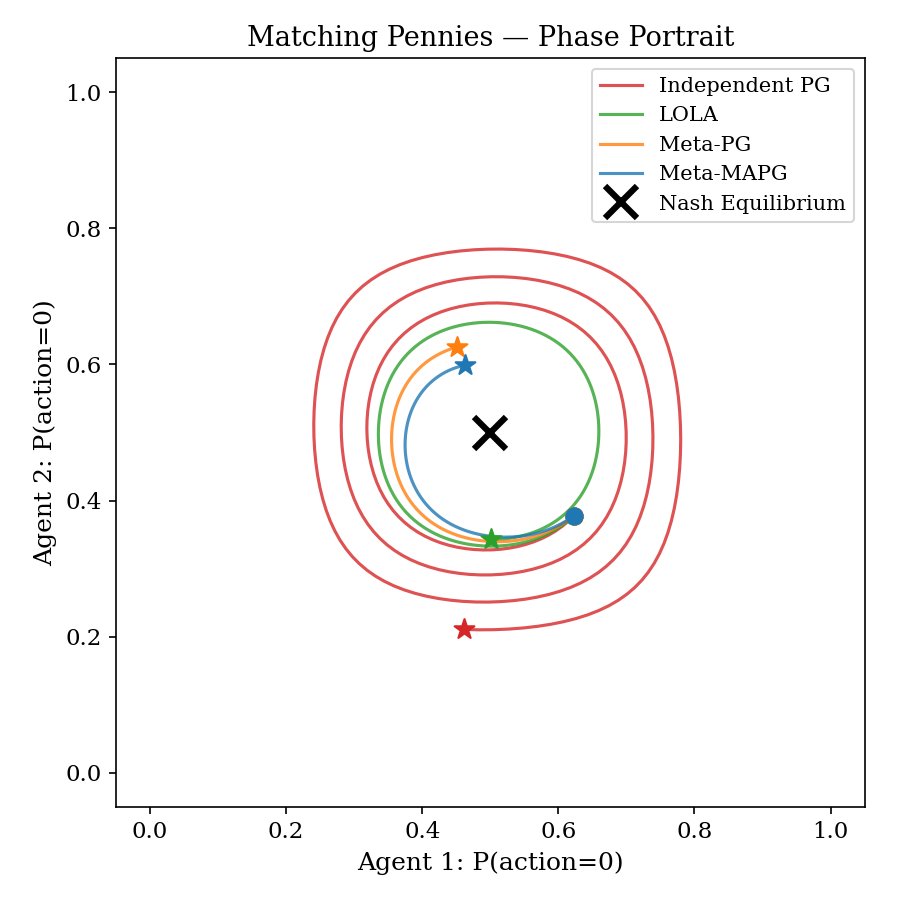
\includegraphics[width=0.55\textwidth]{figures/matching_pennies_phase.png}
\caption{Phase portrait in policy space. Meta-MAPG spirals inward toward Nash (black X). Independent PG spirals outward. LOLA and Meta-PG converge but more slowly.}
\label{fig:mp-phase}
\end{figure}

\textbf{Key result}: In this zero-sum game, anticipating the opponent's learning (Term 3) is essential for Nash convergence. Independent PG, which ignores inter-agent effects entirely, diverges.

\subsection{Experiment 2: Prisoner's Dilemma}

\begin{figure}[H]
\centering
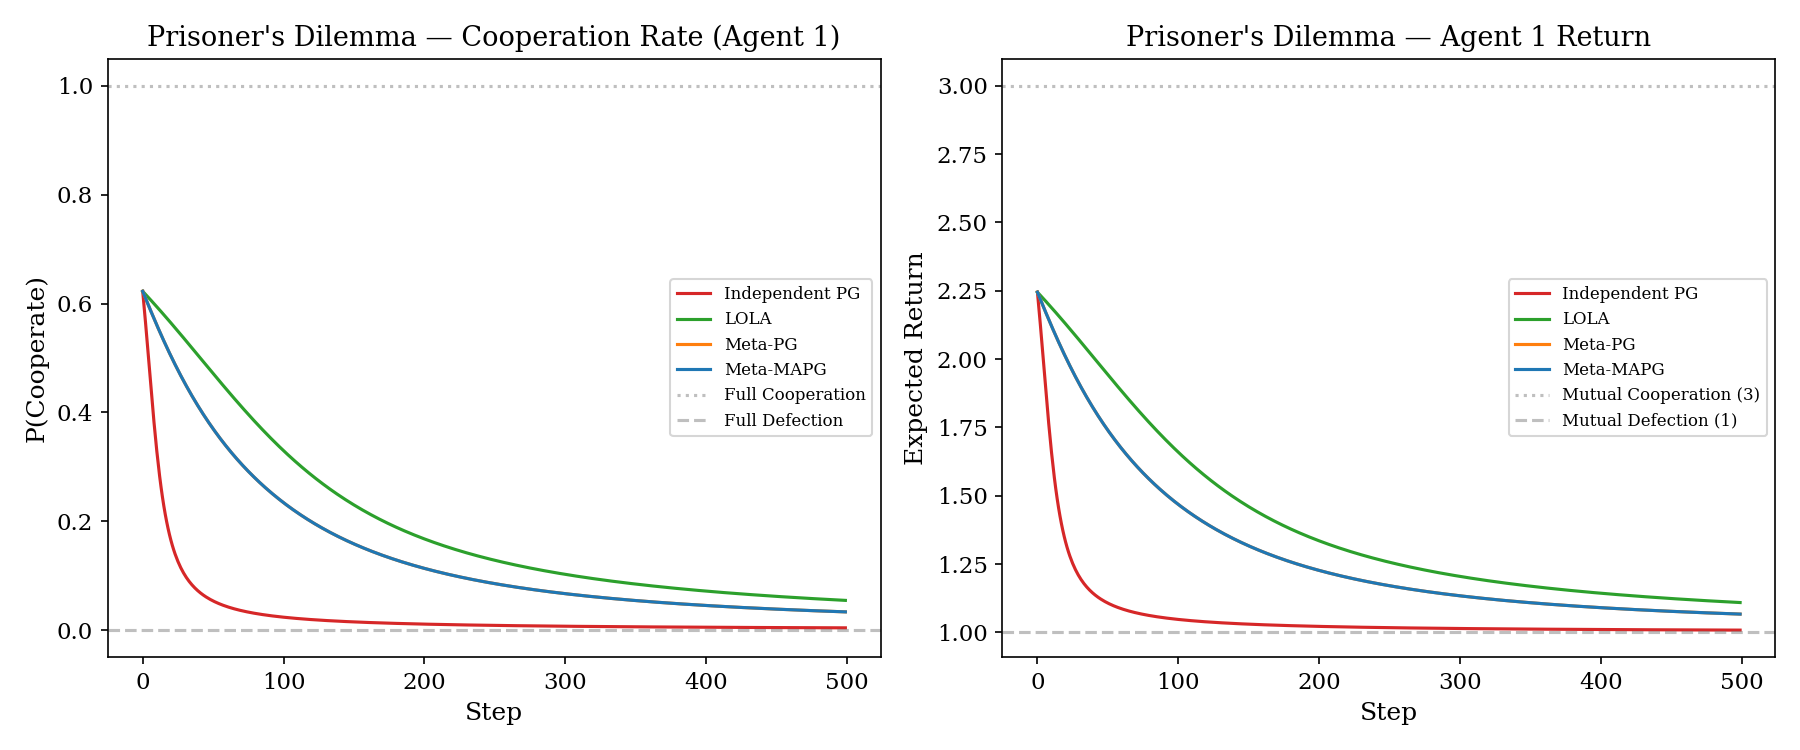
\includegraphics[width=\textwidth]{figures/prisoners_dilemma.png}
\caption{Prisoner's Dilemma. All methods converge to near-defection in this one-shot setting, since $(D, D)$ is the unique Nash equilibrium. Meta-MAPG and Meta-PG achieve marginally higher cooperation ($\approx 5.7\%$) vs.\ Independent PG ($\approx 0.7\%$).}
\label{fig:pd}
\end{figure}

\begin{remark}
The one-shot PD has defection as the dominant strategy. Cooperation emerges only in \emph{iterated} settings with memory, where Term 3 captures the opponent's future response to current cooperation. This limitation is inherent to the stateless game model.
\end{remark}

\subsection{Experiment 3: Lookahead Sensitivity}

\begin{figure}[H]
\centering
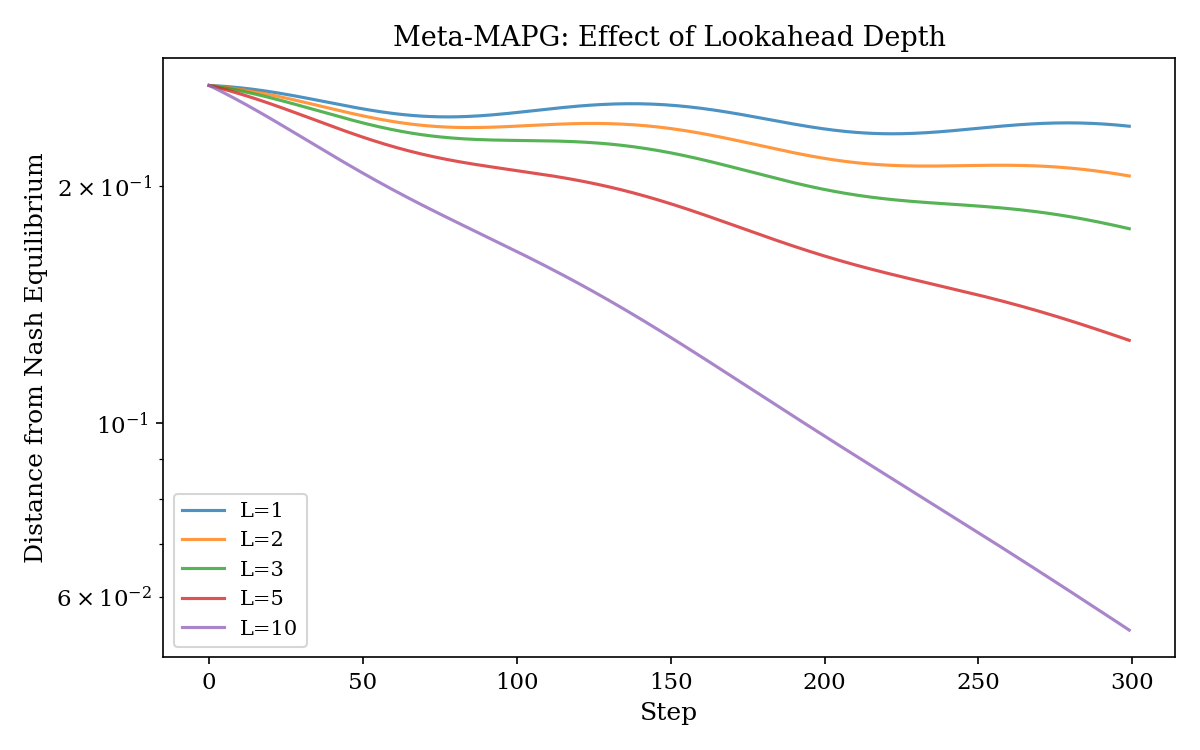
\includegraphics[width=0.65\textwidth]{figures/lookahead_sensitivity.png}
\caption{Effect of lookahead depth $L$ on Meta-MAPG convergence in Matching Pennies. Higher $L$ generally improves convergence speed, with diminishing returns beyond $L = 5$.}
\label{fig:lookahead}
\end{figure}

\subsection{Experiment 4: Initial Condition Robustness}

\begin{figure}[H]
\centering
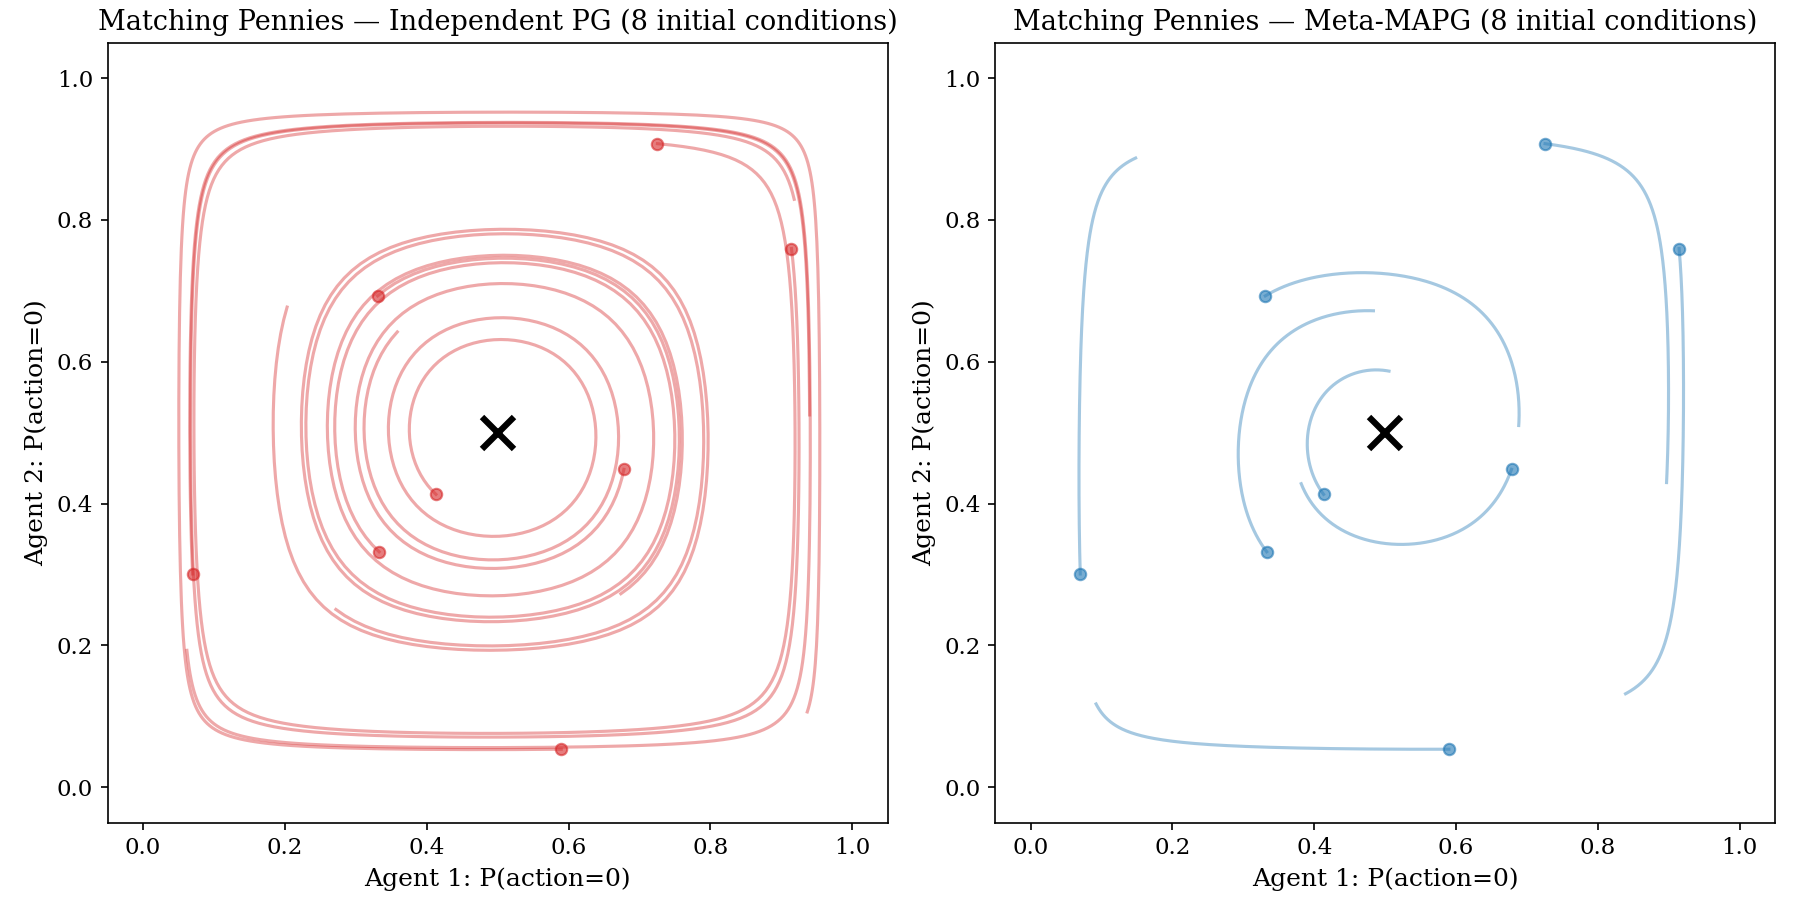
\includegraphics[width=\textwidth]{figures/initial_conditions.png}
\caption{Eight random initial conditions in Matching Pennies. Independent PG trajectories diverge chaotically. Meta-MAPG trajectories all converge toward Nash regardless of initialisation.}
\label{fig:init-cond}
\end{figure}

\subsection{Baseline Numerical Summary}

\begin{center}
\begin{tabular}{llrrrr}
\toprule
\textbf{Game} & \textbf{Method} & $p_1$ & $p_2$ & $V^1$ & $d(\text{Nash})$ \\
\midrule
\multirow{4}{*}{Matching Pennies} & Independent PG & 0.851 & 0.378 & $-0.172$ & 0.371 \\
& LOLA & 0.613 & 0.478 & $-0.010$ & 0.115 \\
& Meta-PG & 0.602 & 0.446 & $-0.022$ & 0.115 \\
& \textbf{Meta-MAPG} & \textbf{0.565} & \textbf{0.463} & $\mathbf{-0.010}$ & \textbf{0.075} \\
\midrule
\multirow{4}{*}{Prisoner's Dilemma} & Independent PG & 0.007 & 0.007 & 1.014 & --- \\
& LOLA & 0.024 & 0.024 & 1.048 & --- \\
& Meta-PG & 0.057 & 0.057 & 1.114 & --- \\
& Meta-MAPG & 0.057 & 0.057 & 1.114 & --- \\
\bottomrule
\end{tabular}
\end{center}

\newpage
% ══════════════════════════════════════════════════════════════════════
\section{Experiment 5: Gradient Term Decomposition}
\label{sec:decomposition}
% ══════════════════════════════════════════════════════════════════════

\textbf{This is the central experiment.} We instrument Meta-MAPG to separately measure the magnitudes of Terms 1, 2, and 3 at each training step, revealing how game structure determines which gradient components drive behaviour.

\begin{figure}[H]
\centering
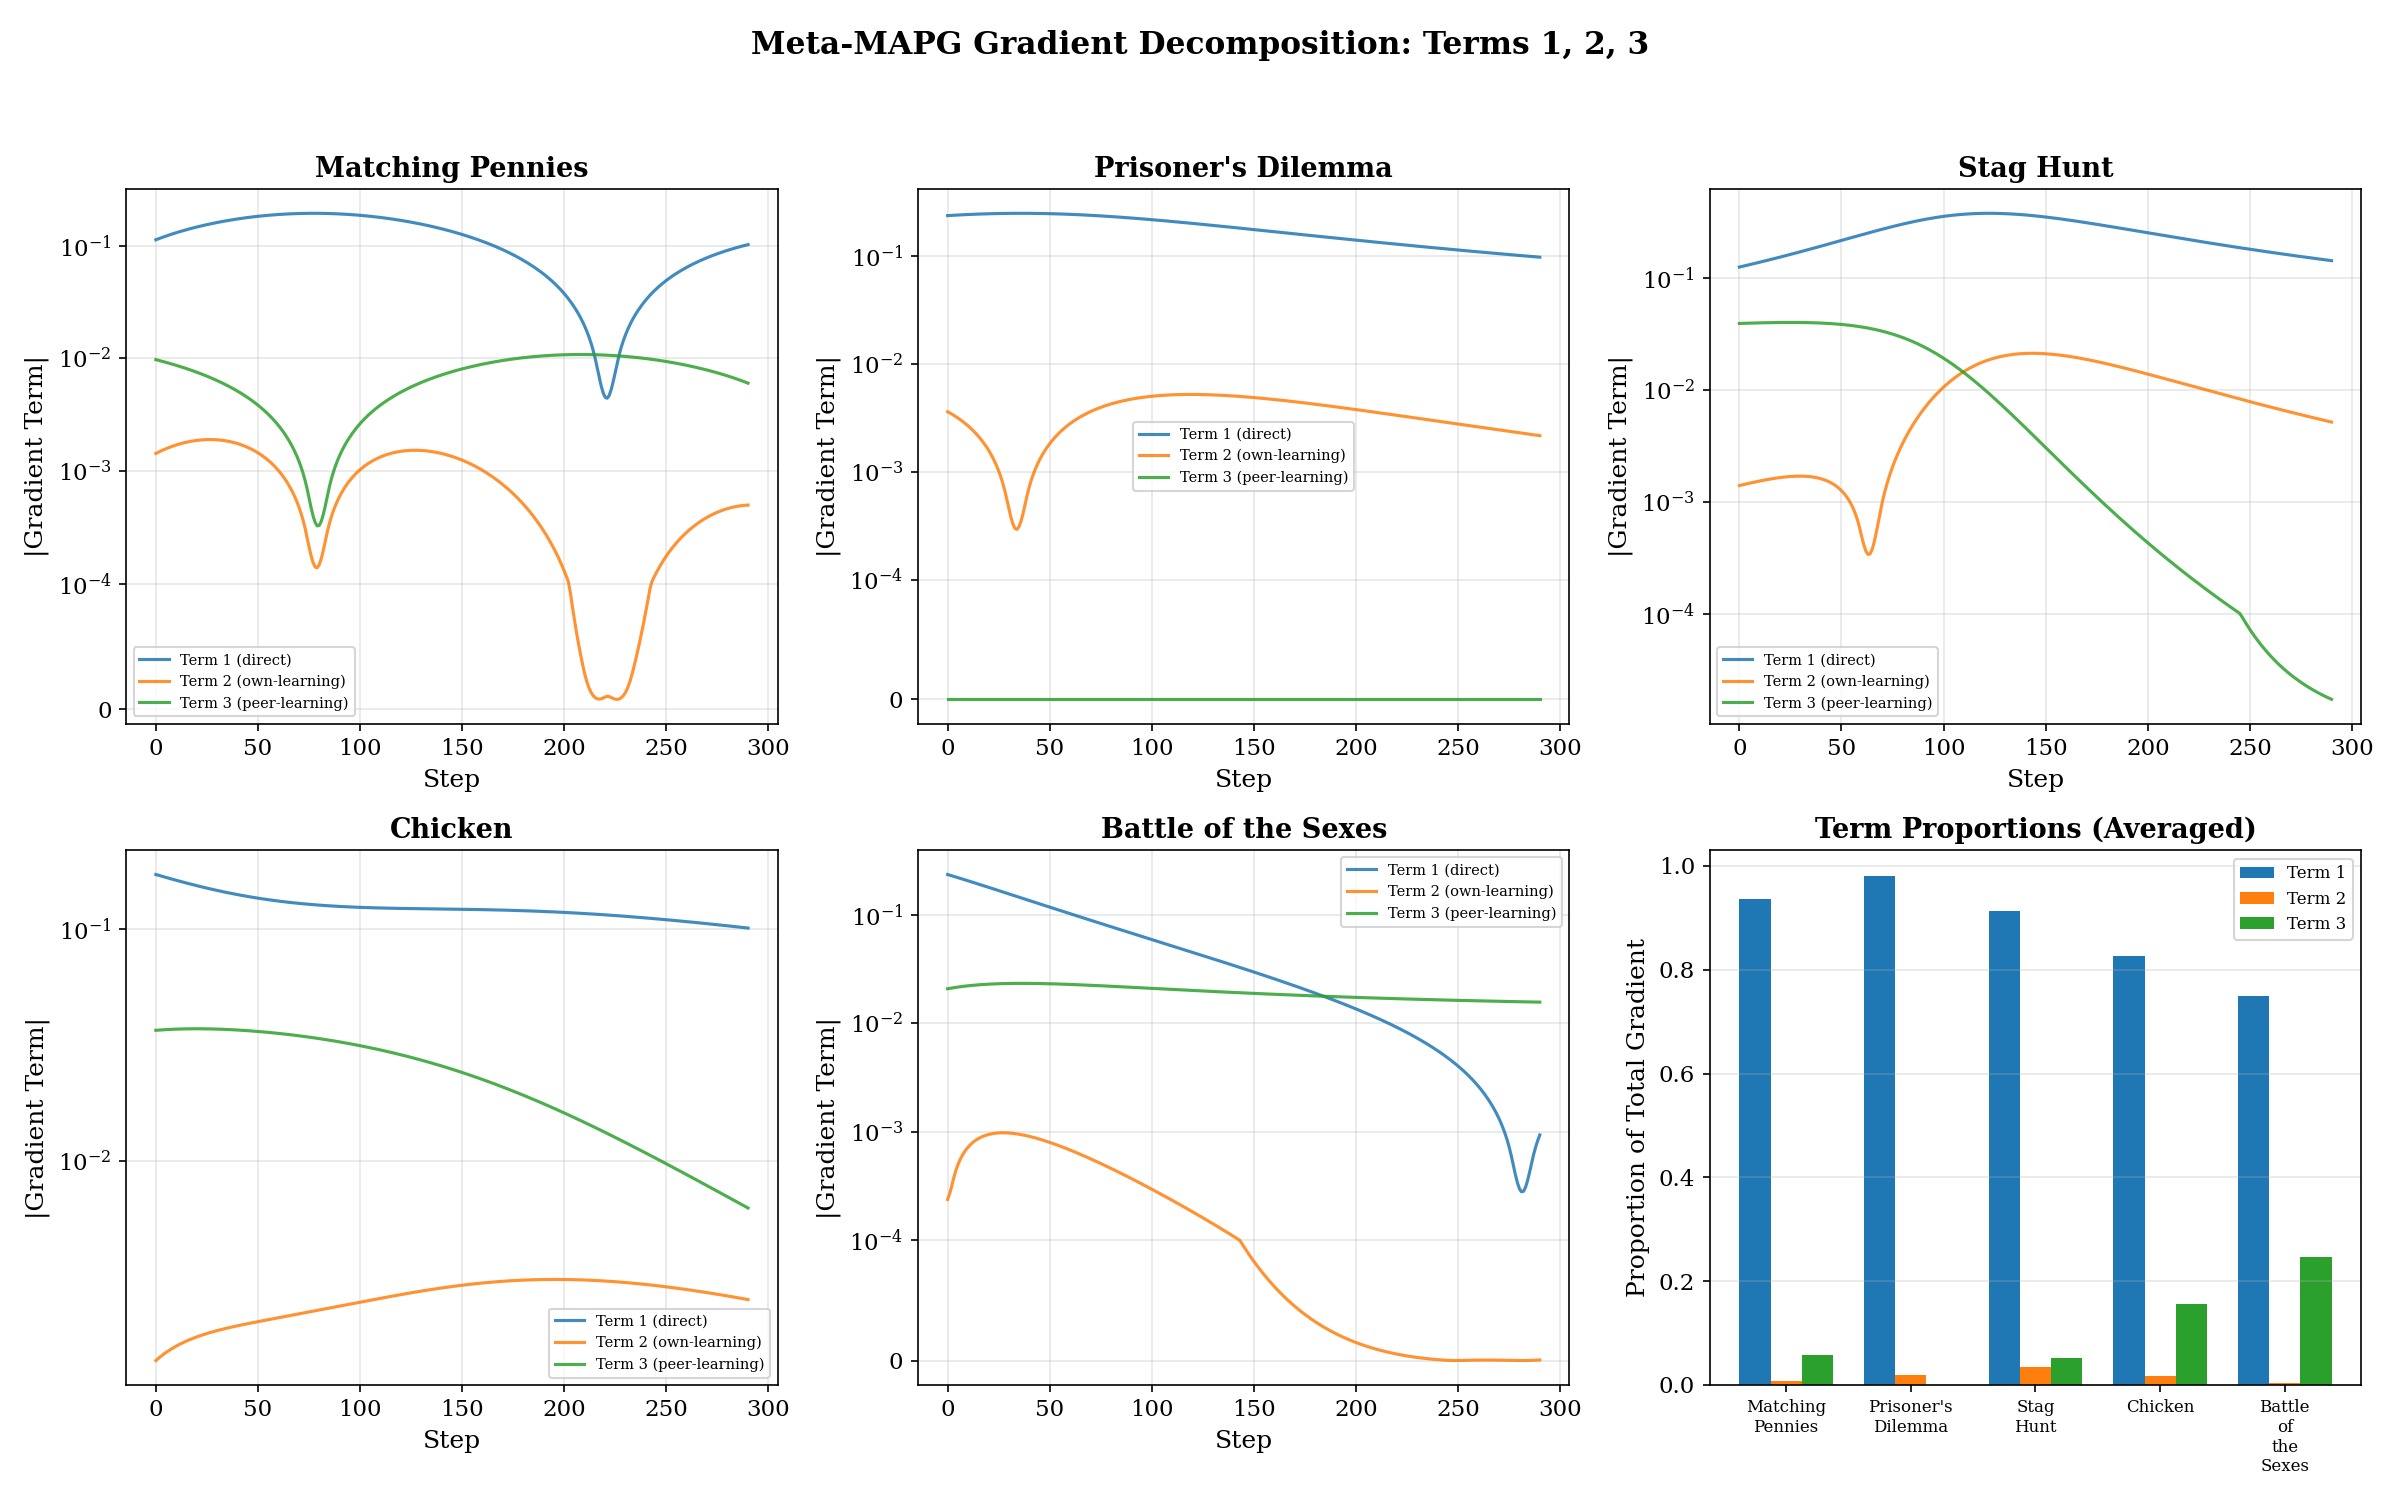
\includegraphics[width=\textwidth]{figures/gradient_decomposition.png}
\caption{Gradient term decomposition across five games. Top-left to bottom-middle: time series of $|\text{Term}|$ on symlog scale. Bottom-right: average proportions. In Matching Pennies, Term 3 (peer-learning) dominates. In Prisoner's Dilemma, Term 1 (direct) accounts for $>80\%$. Chicken shows the most balanced mix.}
\label{fig:decomp}
\end{figure}

\subsection{Interpretation}

\begin{itemize}[nosep]
\item \textbf{Matching Pennies} (zero-sum): Term 3 (peer-learning) is critical. Around step 200, Term 1 drops near zero (approaching Nash), but Term 3 remains active, providing the corrective signal that prevents divergence. This confirms the theoretical prediction: in adversarial settings, modelling the opponent's adaptation is essential.

\item \textbf{Prisoner's Dilemma}: Term 1 overwhelmingly dominates ($>80\%$). Terms 2 and 3 are small because both agents are driven toward the same equilibrium (mutual defection) by their direct gradients. The meta-learning terms have little to ``learn about'' when the game has a dominant strategy.

\item \textbf{Stag Hunt} (coordination): Term 2 (own-learning) grows over training. Agents benefit from anticipating how their current policy affects their own future updates --- the own-learning pathway is how coordination crystallises.

\item \textbf{Chicken} (anti-coordination): The most balanced gradient composition. All three terms contribute meaningfully, reflecting the game's complex incentive structure (agents want to differentiate but also avoid mutual disaster).

\item \textbf{Battle of the Sexes}: Term 3 is the largest proportionally, consistent with the need to anticipate the partner's preferences to coordinate on a shared equilibrium.
\end{itemize}

\begin{remark}[Connection to Agents of Chaos]
The decomposition provides a diagnostic tool for multi-agent LLM systems. Each vulnerability documented in the Agents of Chaos paper (Bau Lab, 2026) corresponds to missing gradient terms: agents that destroyed shared resources (CS1) lacked Term 2 (no anticipation of self-harm); agents that complied with attackers (CS2) lacked Term 3 (no model of how compliance reinforces the attacker's strategy). Agents that \emph{did} coordinate on safety norms (CS16) implicitly computed all three terms.
\end{remark}

\newpage
% ══════════════════════════════════════════════════════════════════════
\section{Experiment 6: Extended Game Suite}
% ══════════════════════════════════════════════════════════════════════

We test all four methods across the three new games.

\begin{figure}[H]
\centering
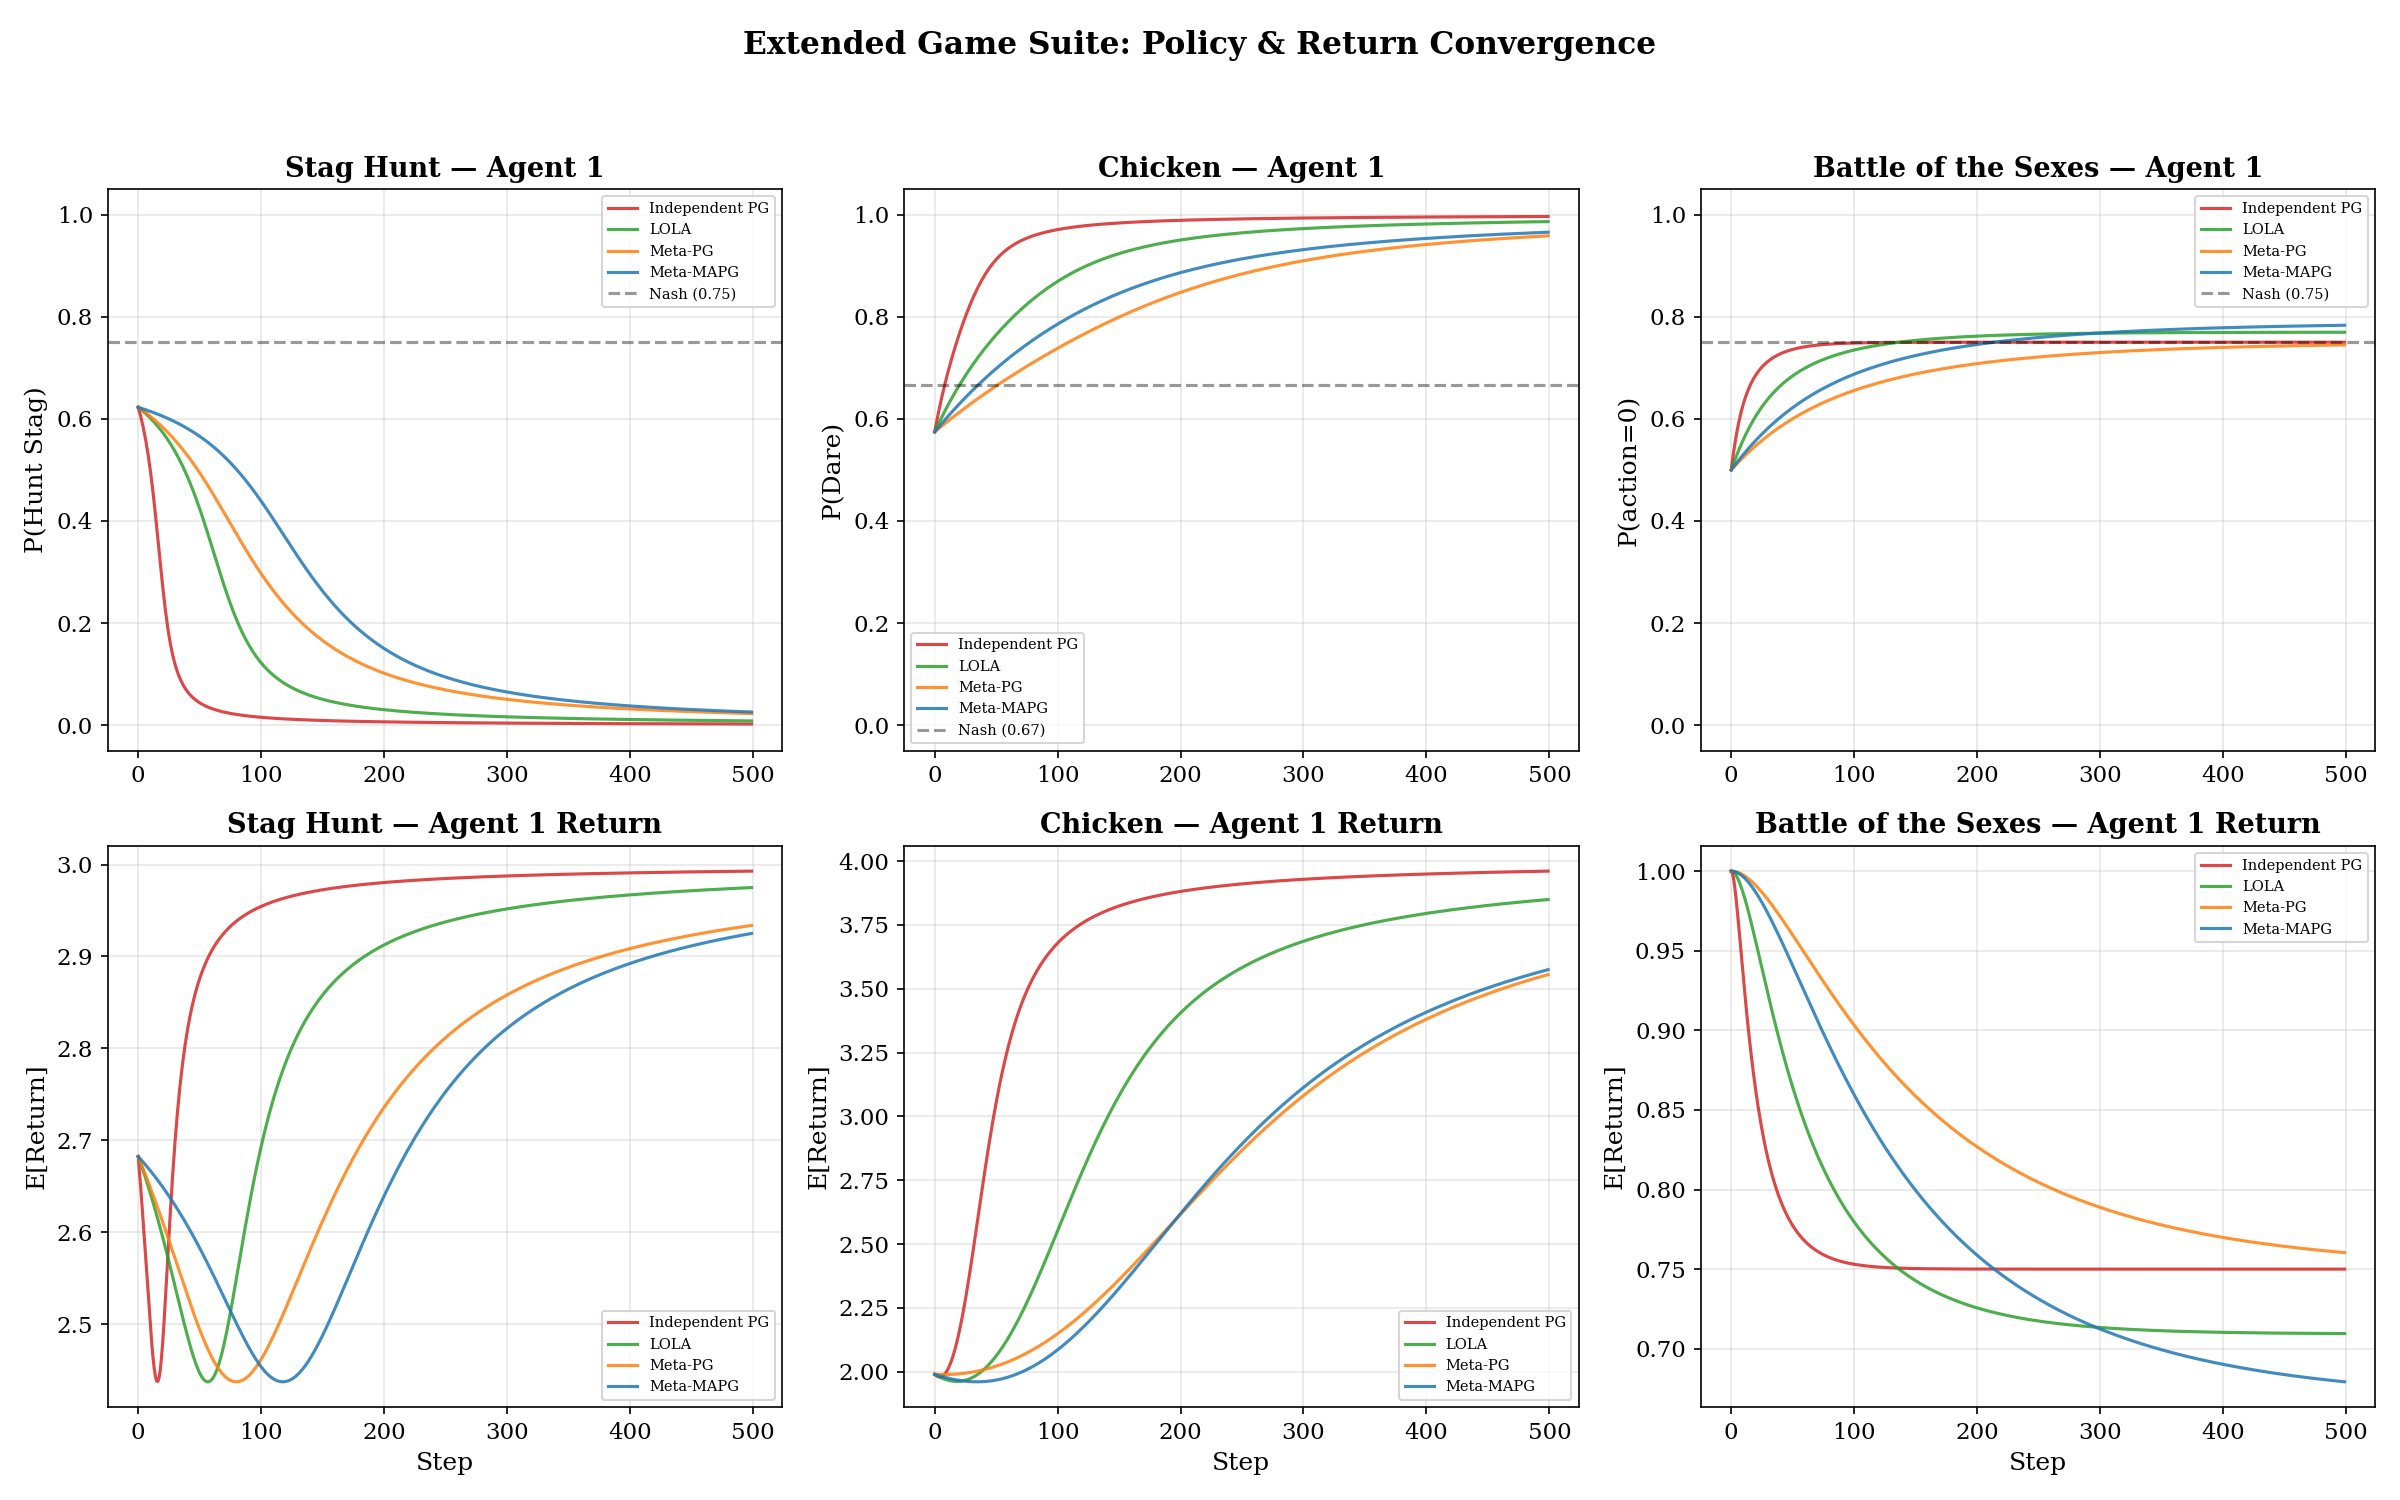
\includegraphics[width=\textwidth]{figures/extended_games.png}
\caption{Policy and return convergence across Stag Hunt, Chicken, and Battle of the Sexes. Top row: Agent 1's policy. Bottom row: Agent 1's expected return.}
\label{fig:extended}
\end{figure}

\textbf{Observations}:
\begin{itemize}[nosep]
\item \textbf{Stag Hunt}: All methods converge to Hare (safe strategy, $p \to 0$), abandoning the payoff-dominant Stag equilibrium. This is the classic risk-dominance result --- agents converge to the safer equilibrium when they cannot trust the partner's cooperation. Meta-MAPG achieves marginally higher cooperation but does not overcome risk-dominance in the stateless setting.

\item \textbf{Chicken}: Agents asymmetrically specialise --- one Dares while the other Swerves. Meta-MAPG and Meta-PG reach higher social welfare than Independent PG.

\item \textbf{Battle of the Sexes}: All methods converge near the mixed Nash $(0.75, 0.25)$. Independent PG converges exactly (the game's gradient landscape naturally funnels toward the mixed NE).
\end{itemize}

\newpage
% ══════════════════════════════════════════════════════════════════════
\section{Experiments 7--8: N-Agent Games}
\label{sec:nagent}
% ══════════════════════════════════════════════════════════════════════

\subsection{Experiment 7: N-Agent Public Goods}

\begin{figure}[H]
\centering
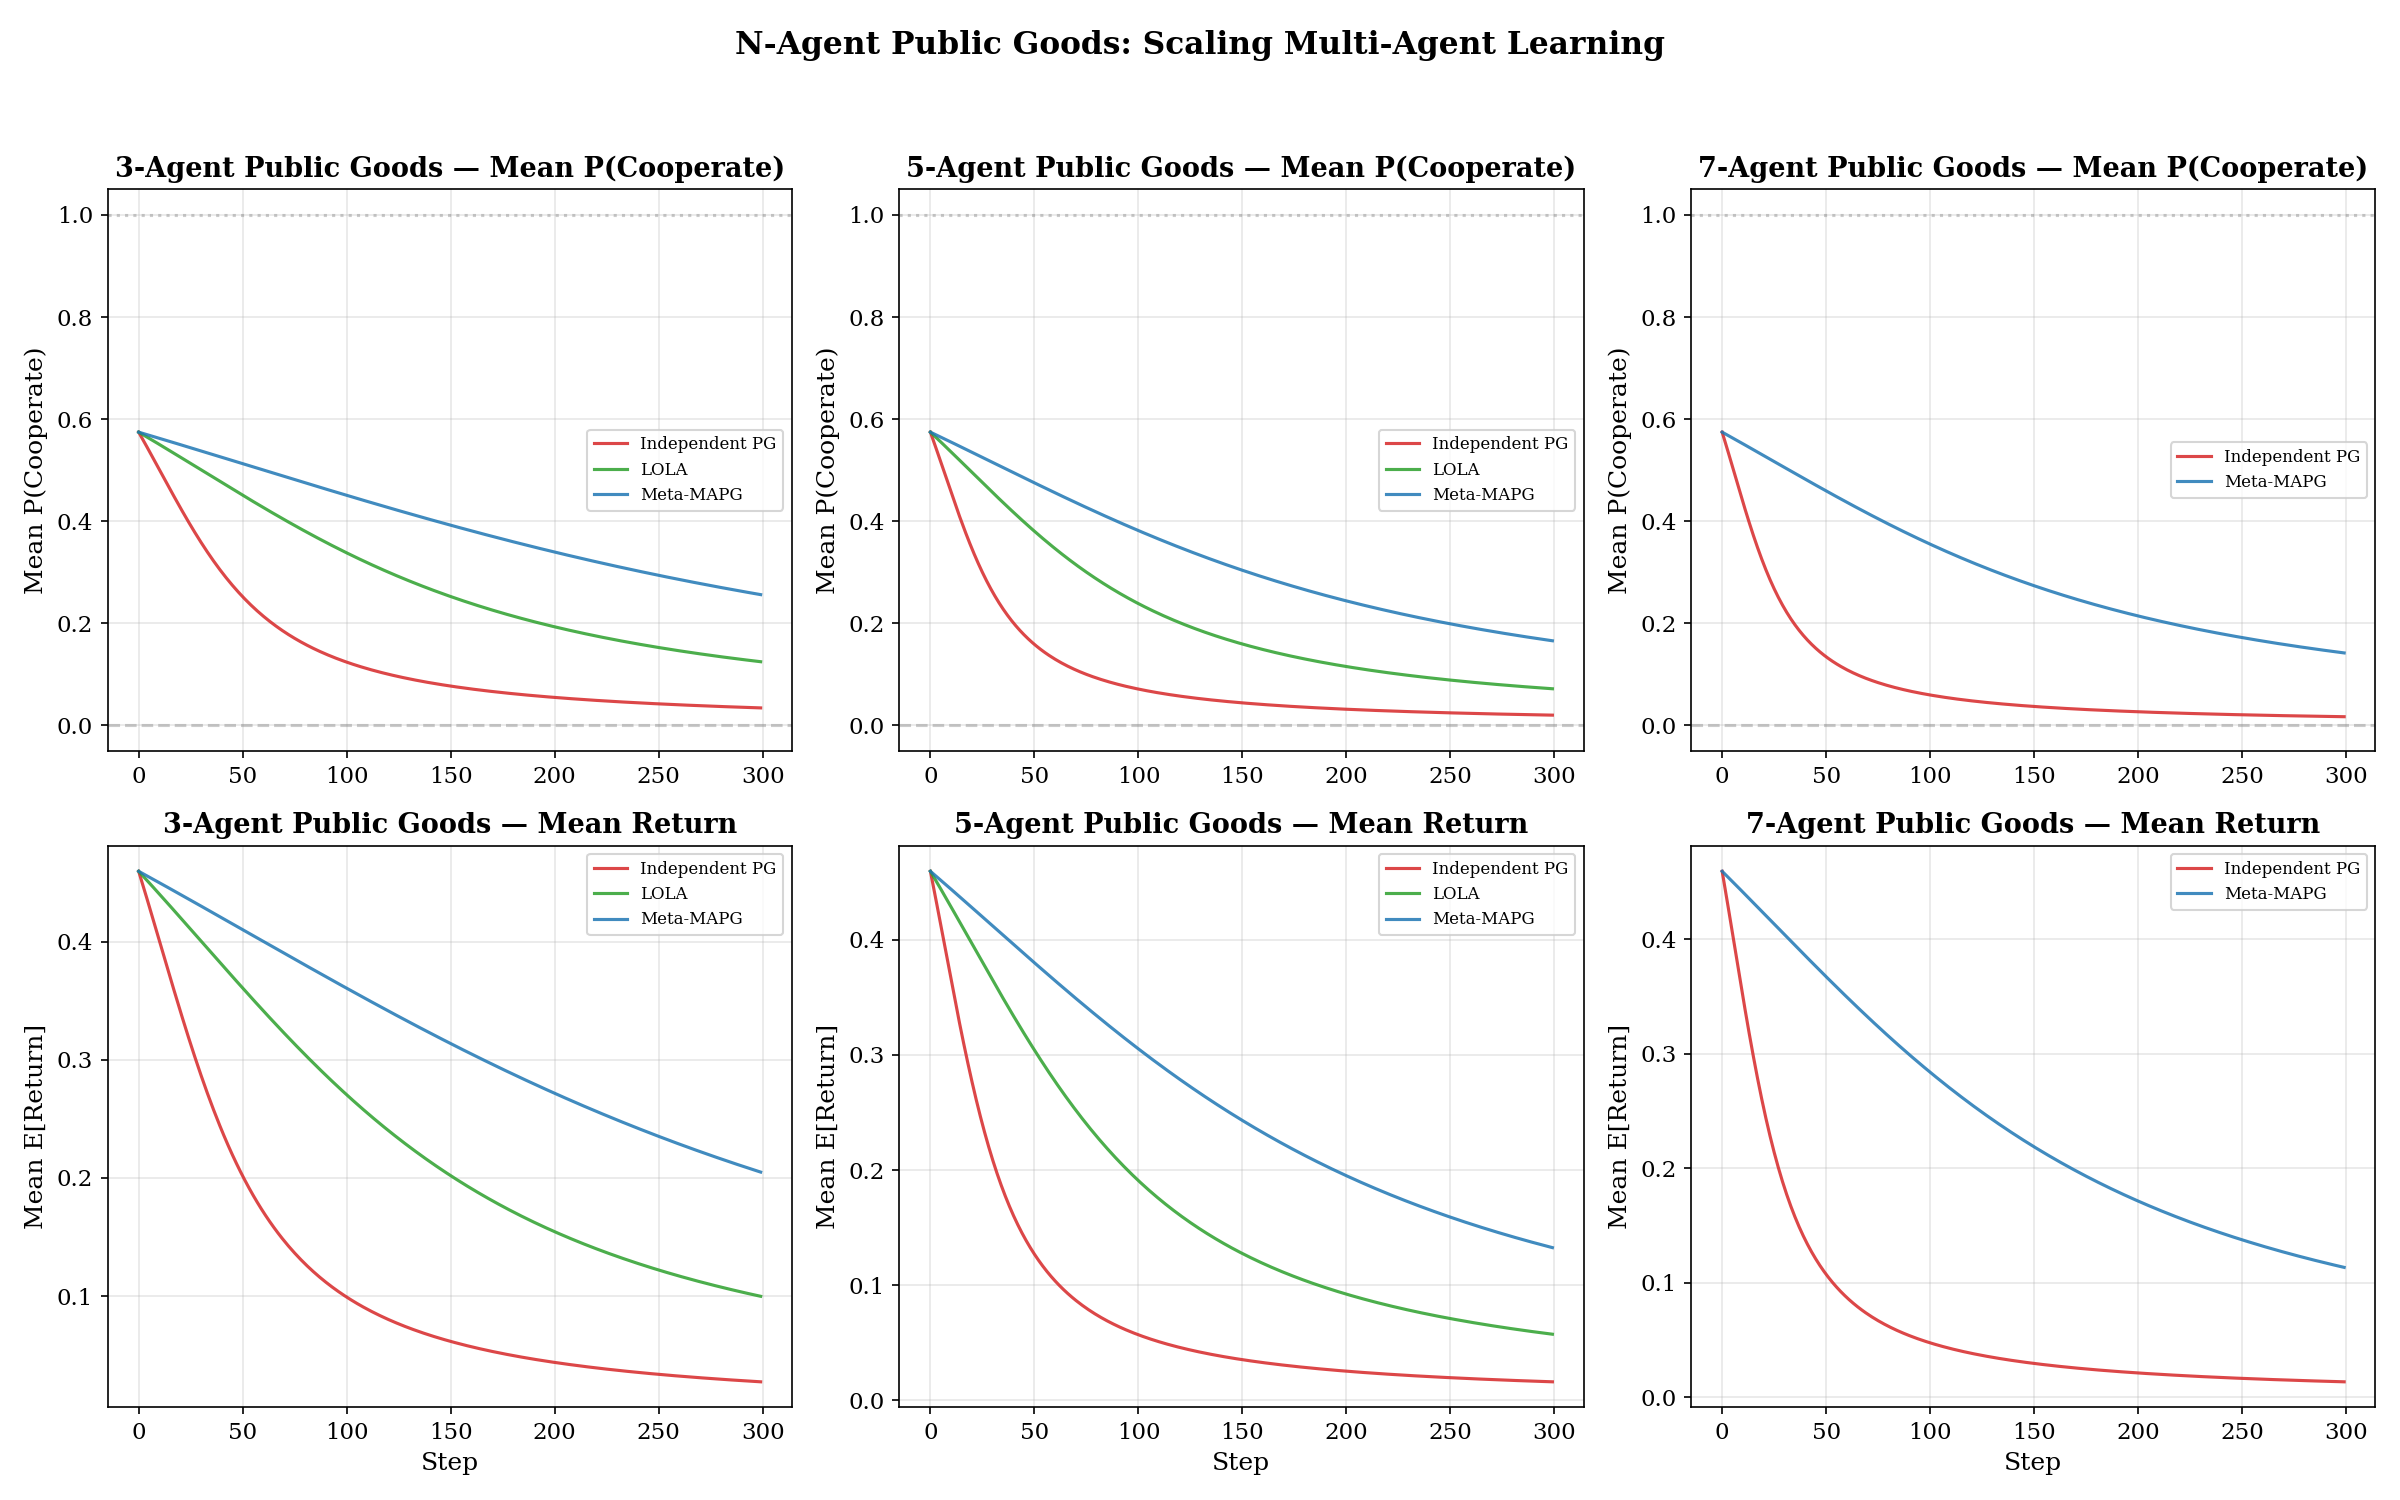
\includegraphics[width=\textwidth]{figures/n_agent_public_goods.png}
\caption{N-Agent Public Goods with $N \in \{3, 5, 7\}$, multiplier $m = 1.8$. Top: mean cooperation probability. Bottom: mean expected return. Meta-MAPG (blue) sustains higher cooperation and returns than Independent PG (red) across all group sizes. LOLA (green, for $N \leq 5$) is intermediate.}
\label{fig:npg}
\end{figure}

\textbf{Key finding}: Meta-MAPG consistently outperforms Independent PG on both cooperation and returns, and the gap \emph{widens} with group size. At $N = 7$, Meta-MAPG's mean return is roughly $2\times$ that of Independent PG after 300 steps. This suggests that the peer-learning term becomes increasingly valuable as the number of interacting agents grows --- directly relevant to multi-agent LLM deployments.

\subsection{Experiment 8: N-Agent Stag Hunt with Thresholds}

\begin{figure}[H]
\centering
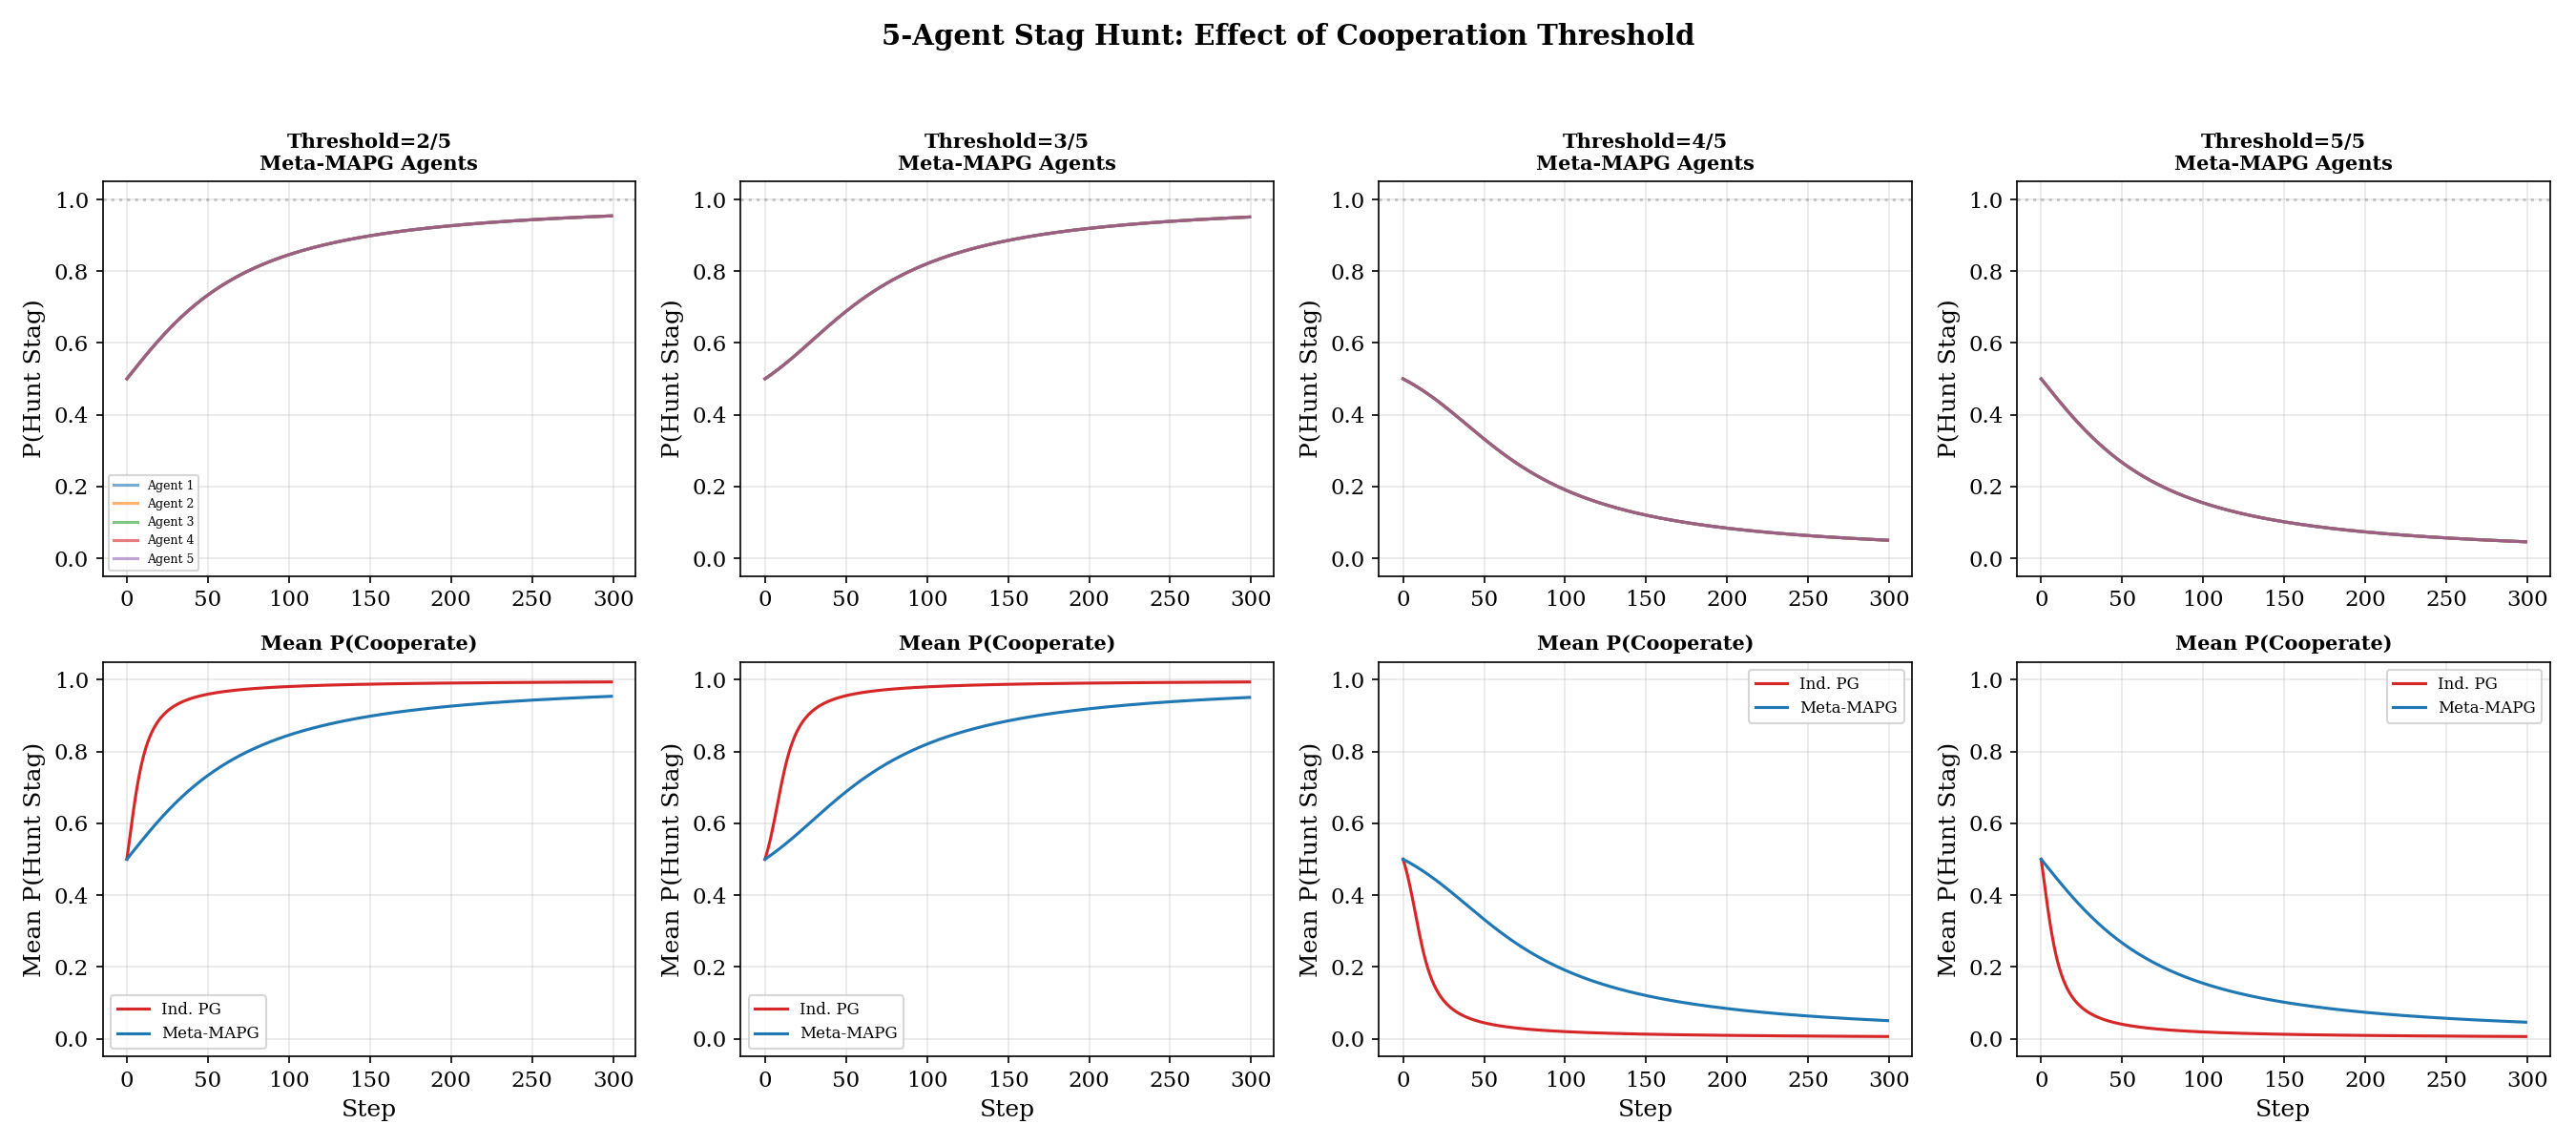
\includegraphics[width=\textwidth]{figures/n_agent_stag_hunt.png}
\caption{5-Agent Stag Hunt with varying cooperation thresholds. Top: individual Meta-MAPG agent trajectories. Bottom: mean cooperation comparison. Lower thresholds ($T = 2, 3$) permit partial cooperation; full unanimity ($T = 5$) prevents it entirely.}
\label{fig:nsh}
\end{figure}

\textbf{Observation}: The threshold acts as a coordination difficulty parameter. When $T = 2$ (only 2 of 5 need to cooperate), Meta-MAPG agents partially coordinate. At $T = 5$ (unanimity required), the risk is too high and all agents defect. This models real-world coordination problems where partial buy-in suffices vs.\ all-or-nothing requirements.

\newpage
% ══════════════════════════════════════════════════════════════════════
\section{Experiment 9: Stochastic vs Exact Gradients}
% ══════════════════════════════════════════════════════════════════════

\begin{figure}[H]
\centering
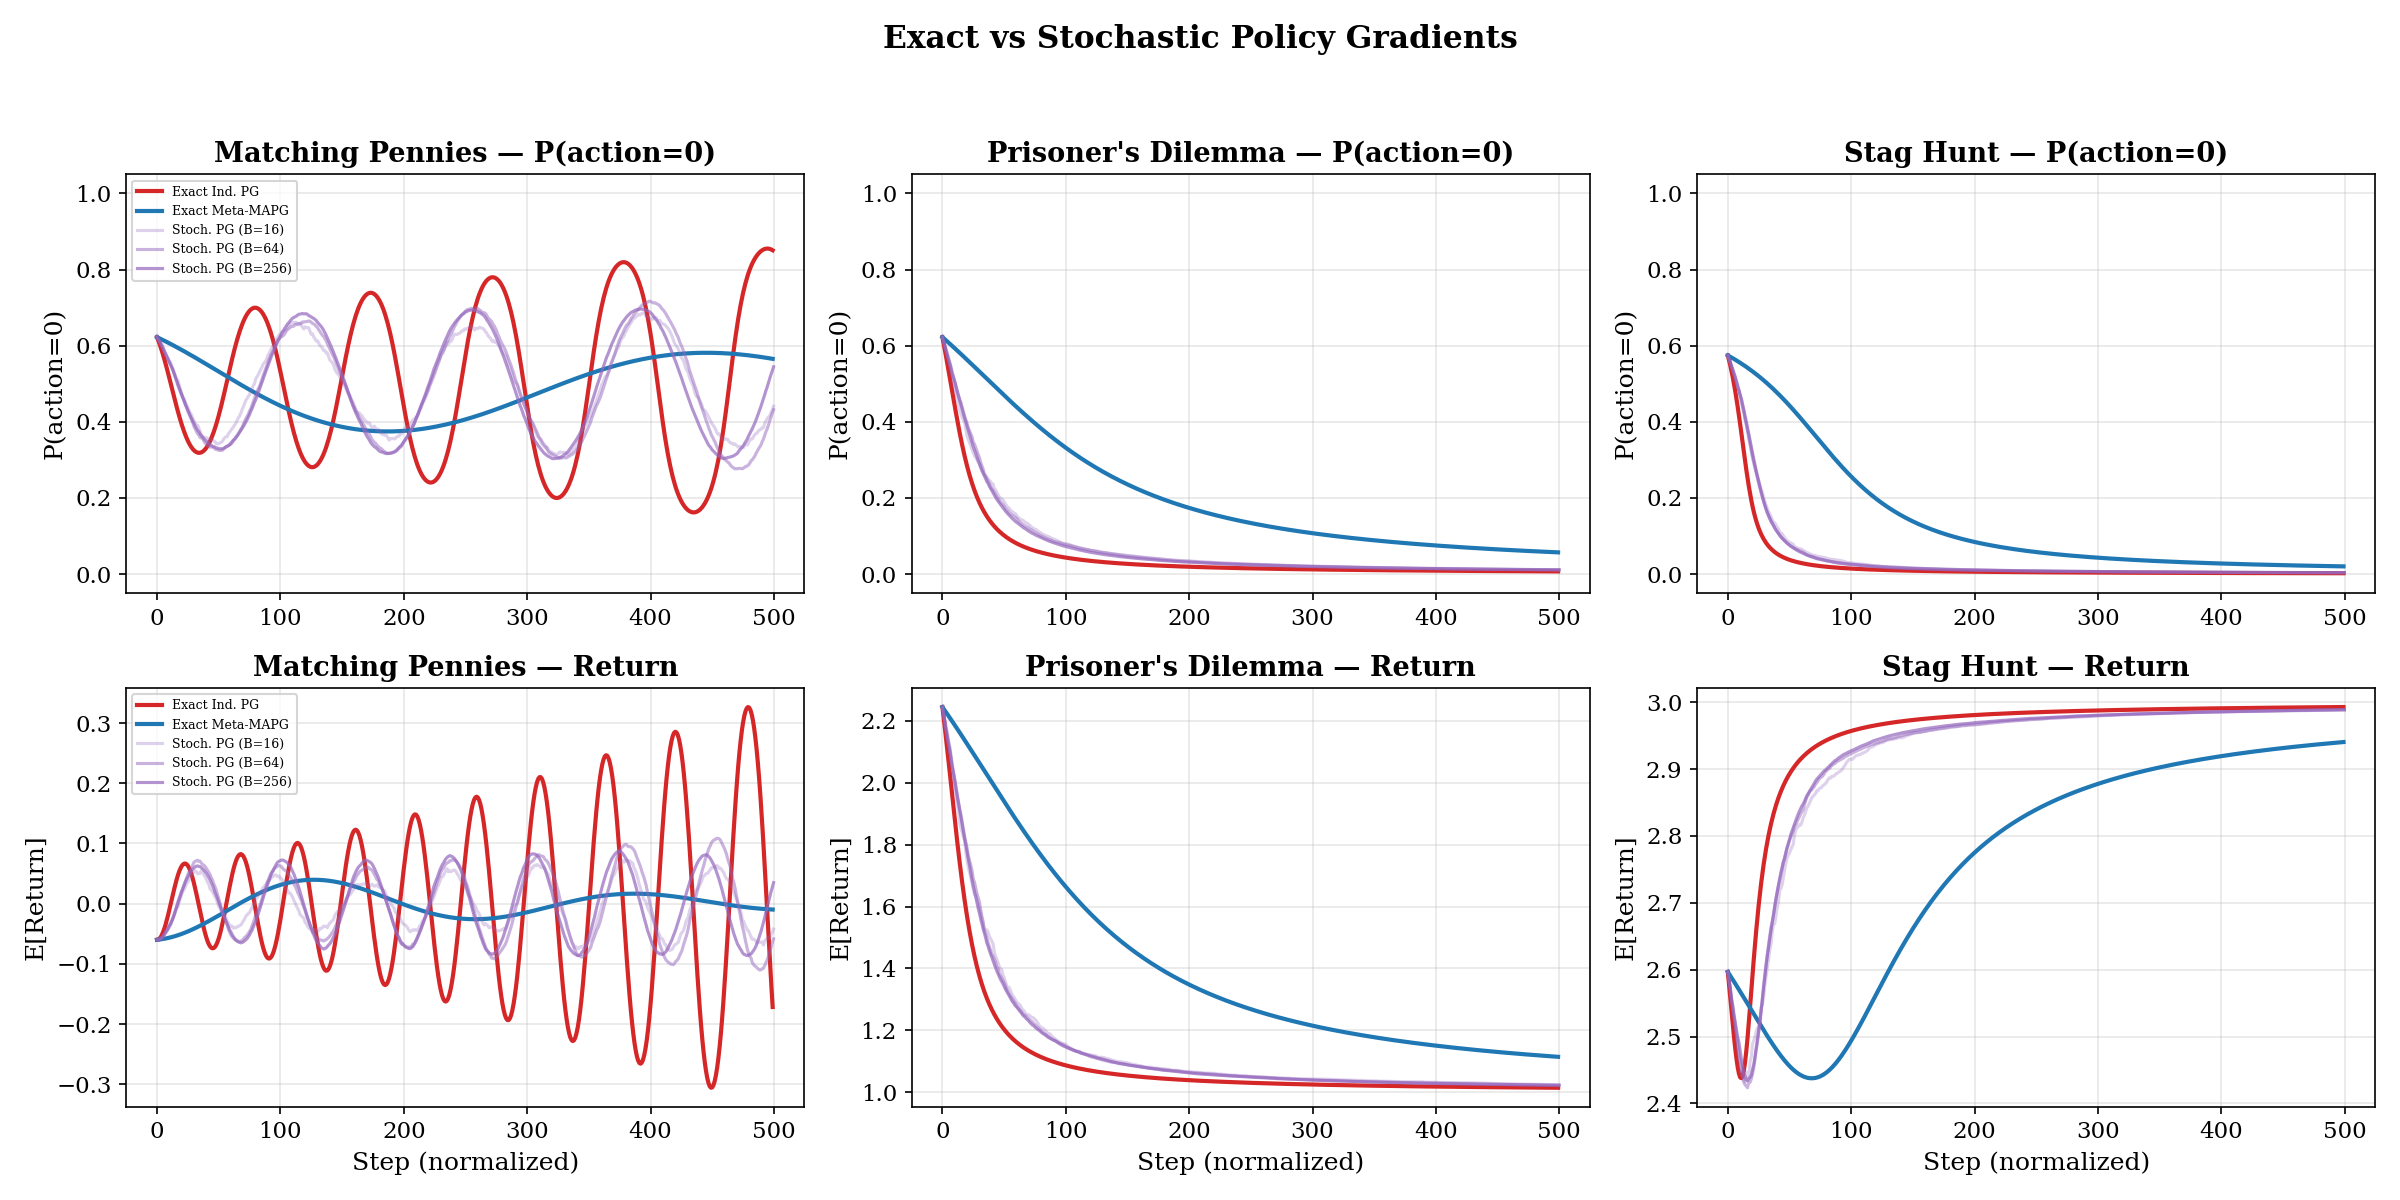
\includegraphics[width=\textwidth]{figures/stochastic_comparison.png}
\caption{Exact analytic gradients vs.\ REINFORCE-based sample gradients at batch sizes $B \in \{16, 64, 256\}$. Stochastic methods converge to the same fixed points but with higher variance and slower speed.}
\label{fig:stochastic}
\end{figure}

The stochastic experiments confirm that the qualitative findings hold under realistic sampling noise. Larger batch sizes reduce variance and approach the exact solution. This is relevant for practical implementation, where exact gradients are unavailable.

\newpage
% ══════════════════════════════════════════════════════════════════════
\section{Experiment 10: Learning Rate Landscape}
% ══════════════════════════════════════════════════════════════════════

\begin{figure}[H]
\centering
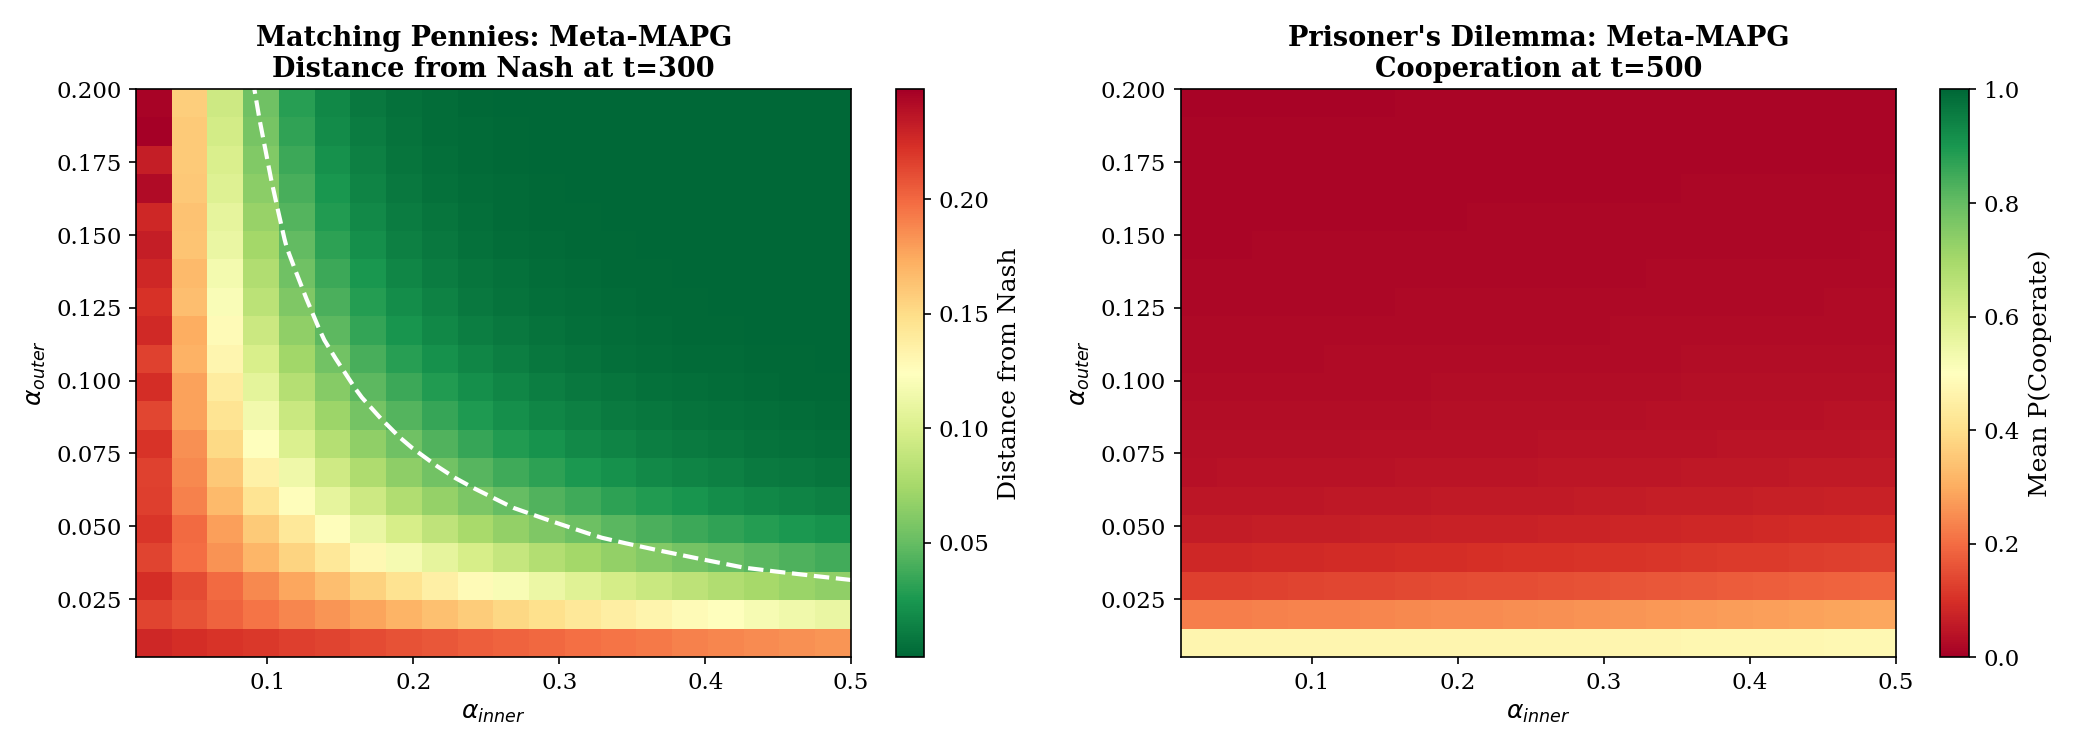
\includegraphics[width=\textwidth]{figures/lr_landscape.png}
\caption{Left: Meta-MAPG distance from Nash in Matching Pennies as a function of $(\alpha_\text{inner}, \alpha_\text{outer})$, with white contour at $d < 0.05$. The stable region requires $\alpha_\text{inner} \gtrsim 0.1$. Right: Cooperation level in Prisoner's Dilemma --- uniformly low, confirming the one-shot limitation.}
\label{fig:lr}
\end{figure}

\textbf{Key finding}: Meta-MAPG's convergence in Matching Pennies is robust across a wide range of hyperparameters, with the stable region (inside white contour) covering most of the $\alpha_\text{inner} > 0.1$ half-plane. Very small inner learning rates ($\alpha_\text{inner} < 0.05$) cause instability because the inner-loop steps are too small to produce meaningful Jacobian information.

\newpage
% ══════════════════════════════════════════════════════════════════════
\section{Experiment 11: Convergence Rate Quantification}
% ══════════════════════════════════════════════════════════════════════

\begin{figure}[H]
\centering
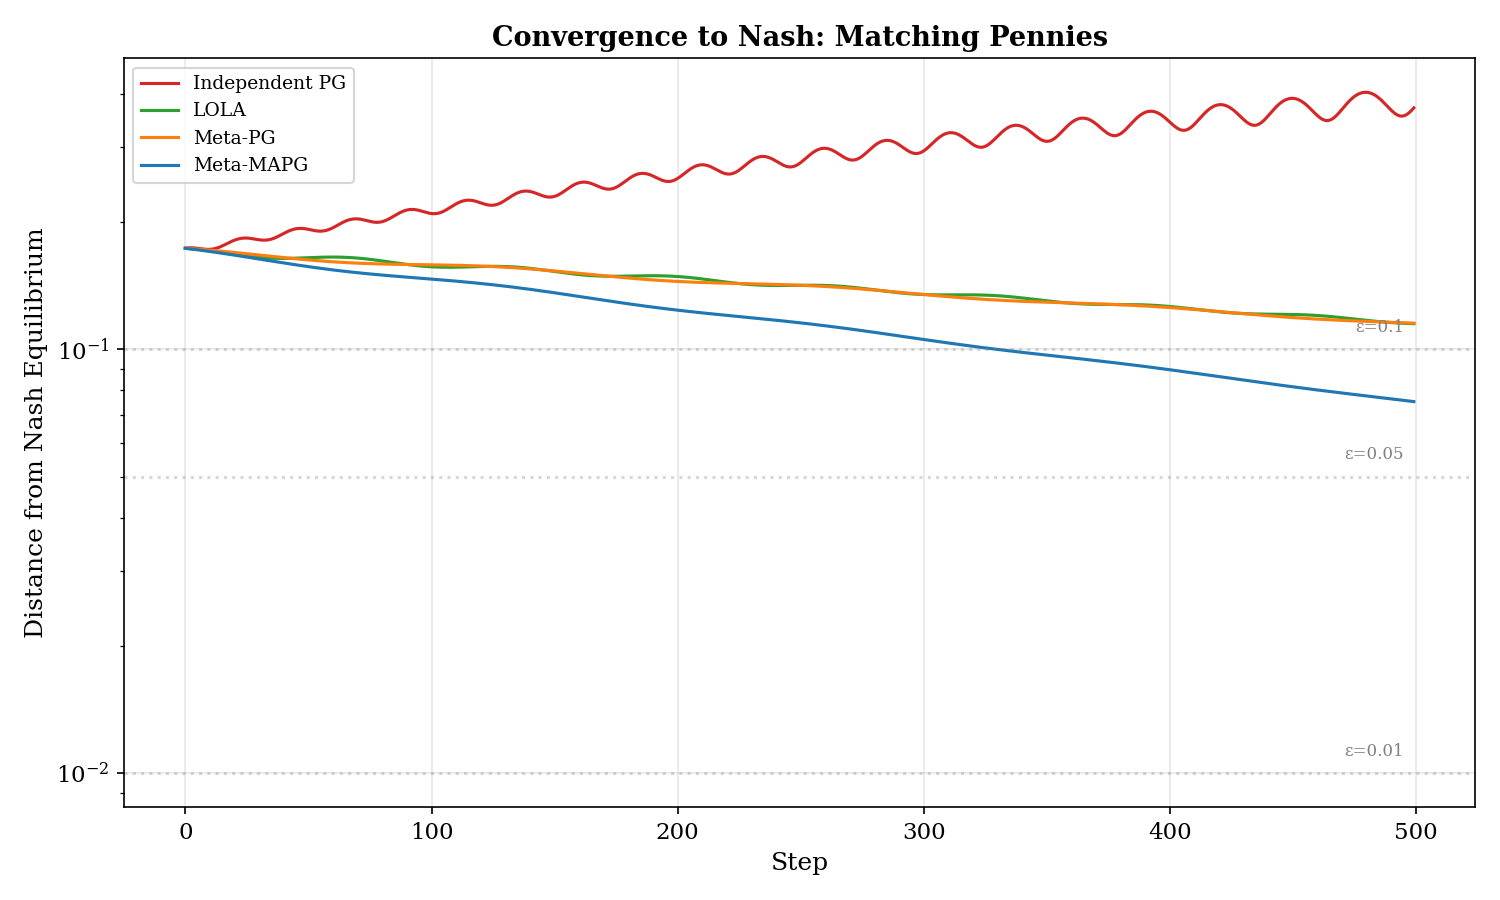
\includegraphics[width=0.7\textwidth]{figures/convergence_rates.png}
\caption{Distance from Nash equilibrium over time (log scale). Meta-MAPG is the only method to enter the $\varepsilon = 0.1$ ball.}
\label{fig:conv}
\end{figure}

\begin{center}
\begin{tabular}{lrrrcc}
\toprule
\textbf{Method} & $T(\varepsilon{=}0.1)$ & $T(\varepsilon{=}0.05)$ & $T(\varepsilon{=}0.01)$ & \textbf{Decay Rate} & \textbf{Final $d$} \\
\midrule
Independent PG & DNR & DNR & DNR & $-0.0012$ & 0.371 \\
LOLA & DNR & DNR & DNR & 0.0008 & 0.115 \\
Meta-PG & DNR & DNR & DNR & 0.0008 & 0.115 \\
\textbf{Meta-MAPG} & \textbf{330} & DNR & DNR & \textbf{0.0017} & \textbf{0.075} \\
\bottomrule
\end{tabular}
\end{center}

\noindent $T(\varepsilon)$ = first step where distance from Nash $< \varepsilon$. DNR = did not reach. Decay rate = negative slope of $\log(\text{distance})$ in the second half of training. Independent PG has a \emph{negative} rate (diverging).

\newpage
% ══════════════════════════════════════════════════════════════════════
\section{Experiments 12--13: Term Dynamics and Jacobian Evolution}
% ══════════════════════════════════════════════════════════════════════

\subsection{Experiment 12: Stacked Area --- Term Proportions Over Time}

\begin{figure}[H]
\centering
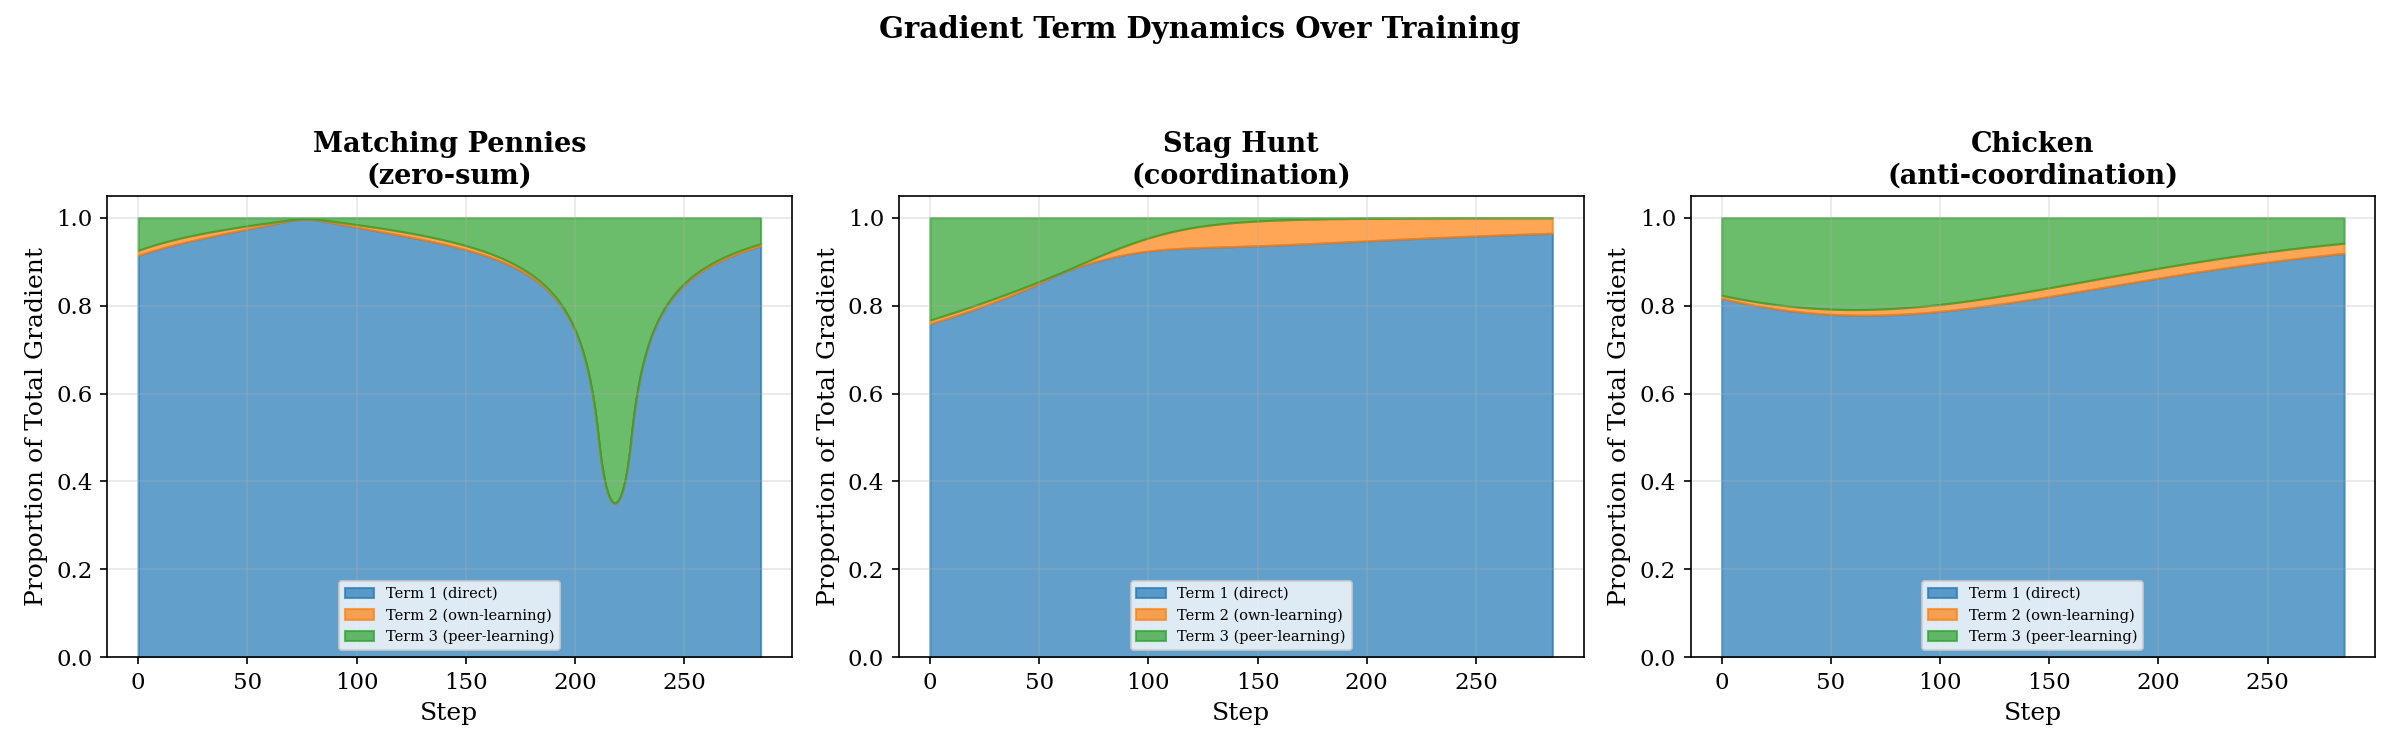
\includegraphics[width=\textwidth]{figures/term_dynamics.png}
\caption{Stacked area chart of gradient term proportions over training. Left: Matching Pennies --- Term 3 (green) surges around step 200 when Term 1 drops near zero. Centre: Stag Hunt --- Term 2 (orange) gradually grows. Right: Chicken --- relatively stable mix with Term 3 growing late.}
\label{fig:dynamics}
\end{figure}

\textbf{Insight}: The gradient composition is not static --- it evolves as agents approach equilibrium. In Matching Pennies, the ``phase transition'' around step 200 is particularly striking: the direct gradient (Term 1) approaches zero as policies near Nash, and the peer-learning term (Term 3) becomes the dominant signal keeping the system on track. This suggests that \emph{different mechanisms matter at different stages of learning}.

\subsection{Experiment 13: Jacobian Evolution}

\begin{figure}[H]
\centering
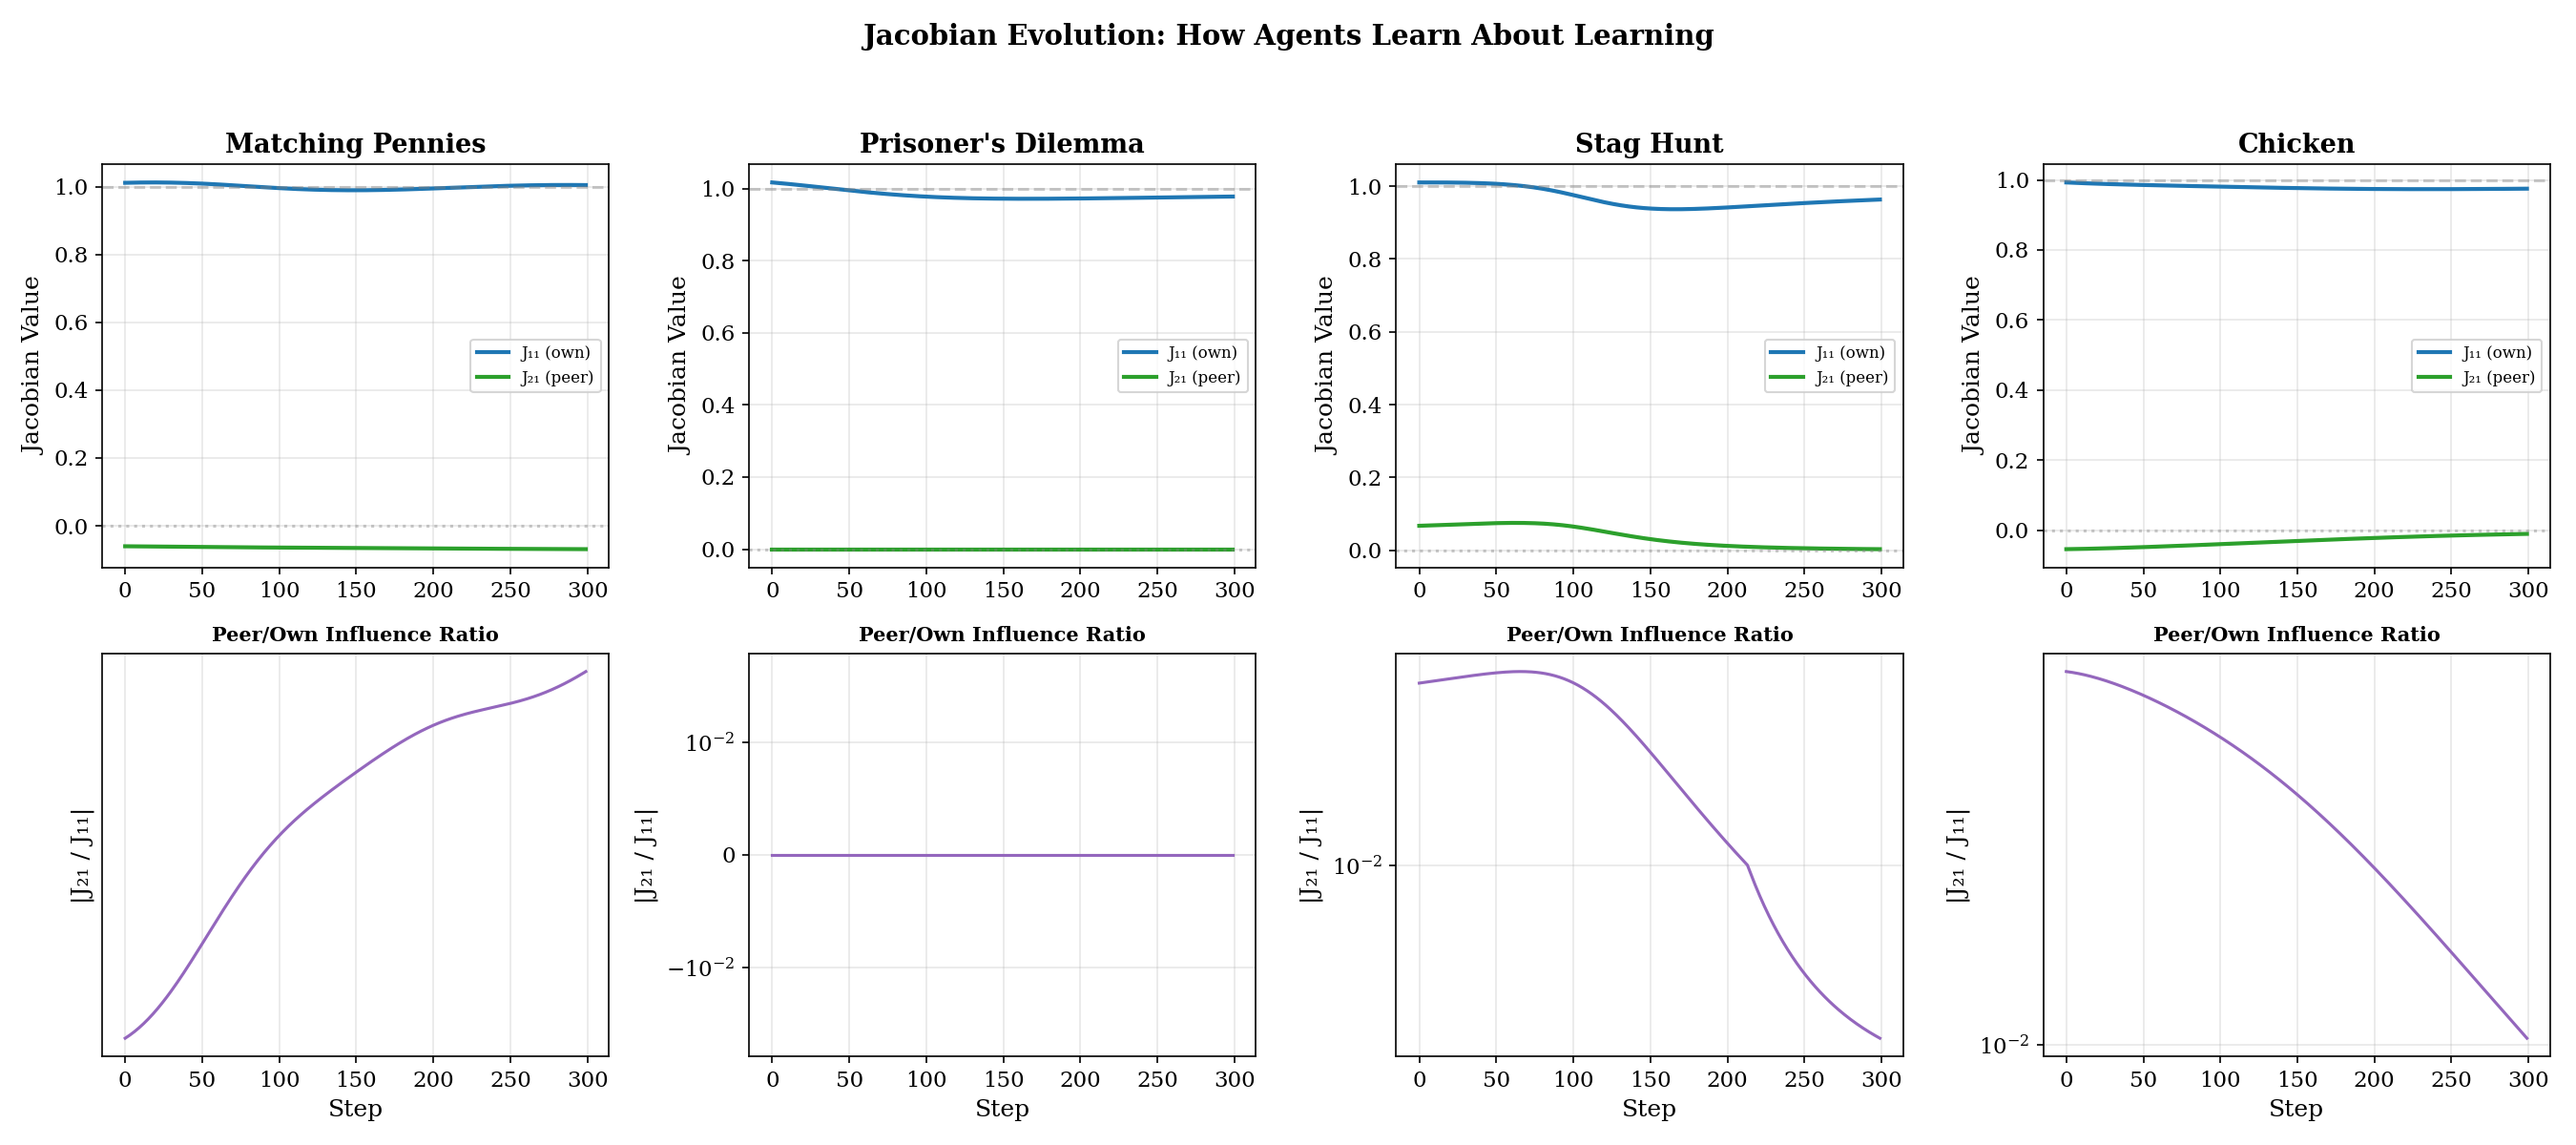
\includegraphics[width=\textwidth]{figures/jacobian_evolution.png}
\caption{Top: Jacobian values $J_{11}$ (own-learning) and $J_{21}$ (peer-learning) over training. Bottom: peer/own influence ratio $|J_{21}/J_{11}|$.}
\label{fig:jacobian}
\end{figure}

The Jacobians track ``how much agent 1's initial parameters affect each agent's parameters after the inner loop.'' Key observations:
\begin{itemize}[nosep]
\item $J_{11} \approx 1$ throughout (own-learning corrections are small perturbations to the identity).
\item $J_{21}$ is small but \emph{consistently negative} in Matching Pennies --- agent 1's parameters push agent 2's parameters in the opposite direction, as expected in a zero-sum game.
\item The peer/own ratio $|J_{21}/J_{11}|$ grows over time in Matching Pennies (reaching $\sim 0.1$), reflecting increasing inter-agent coupling as policies converge.
\end{itemize}

\newpage
% ══════════════════════════════════════════════════════════════════════
\section{Experiment 14: Ablation Study}
% ══════════════════════════════════════════════════════════════════════

\begin{figure}[H]
\centering
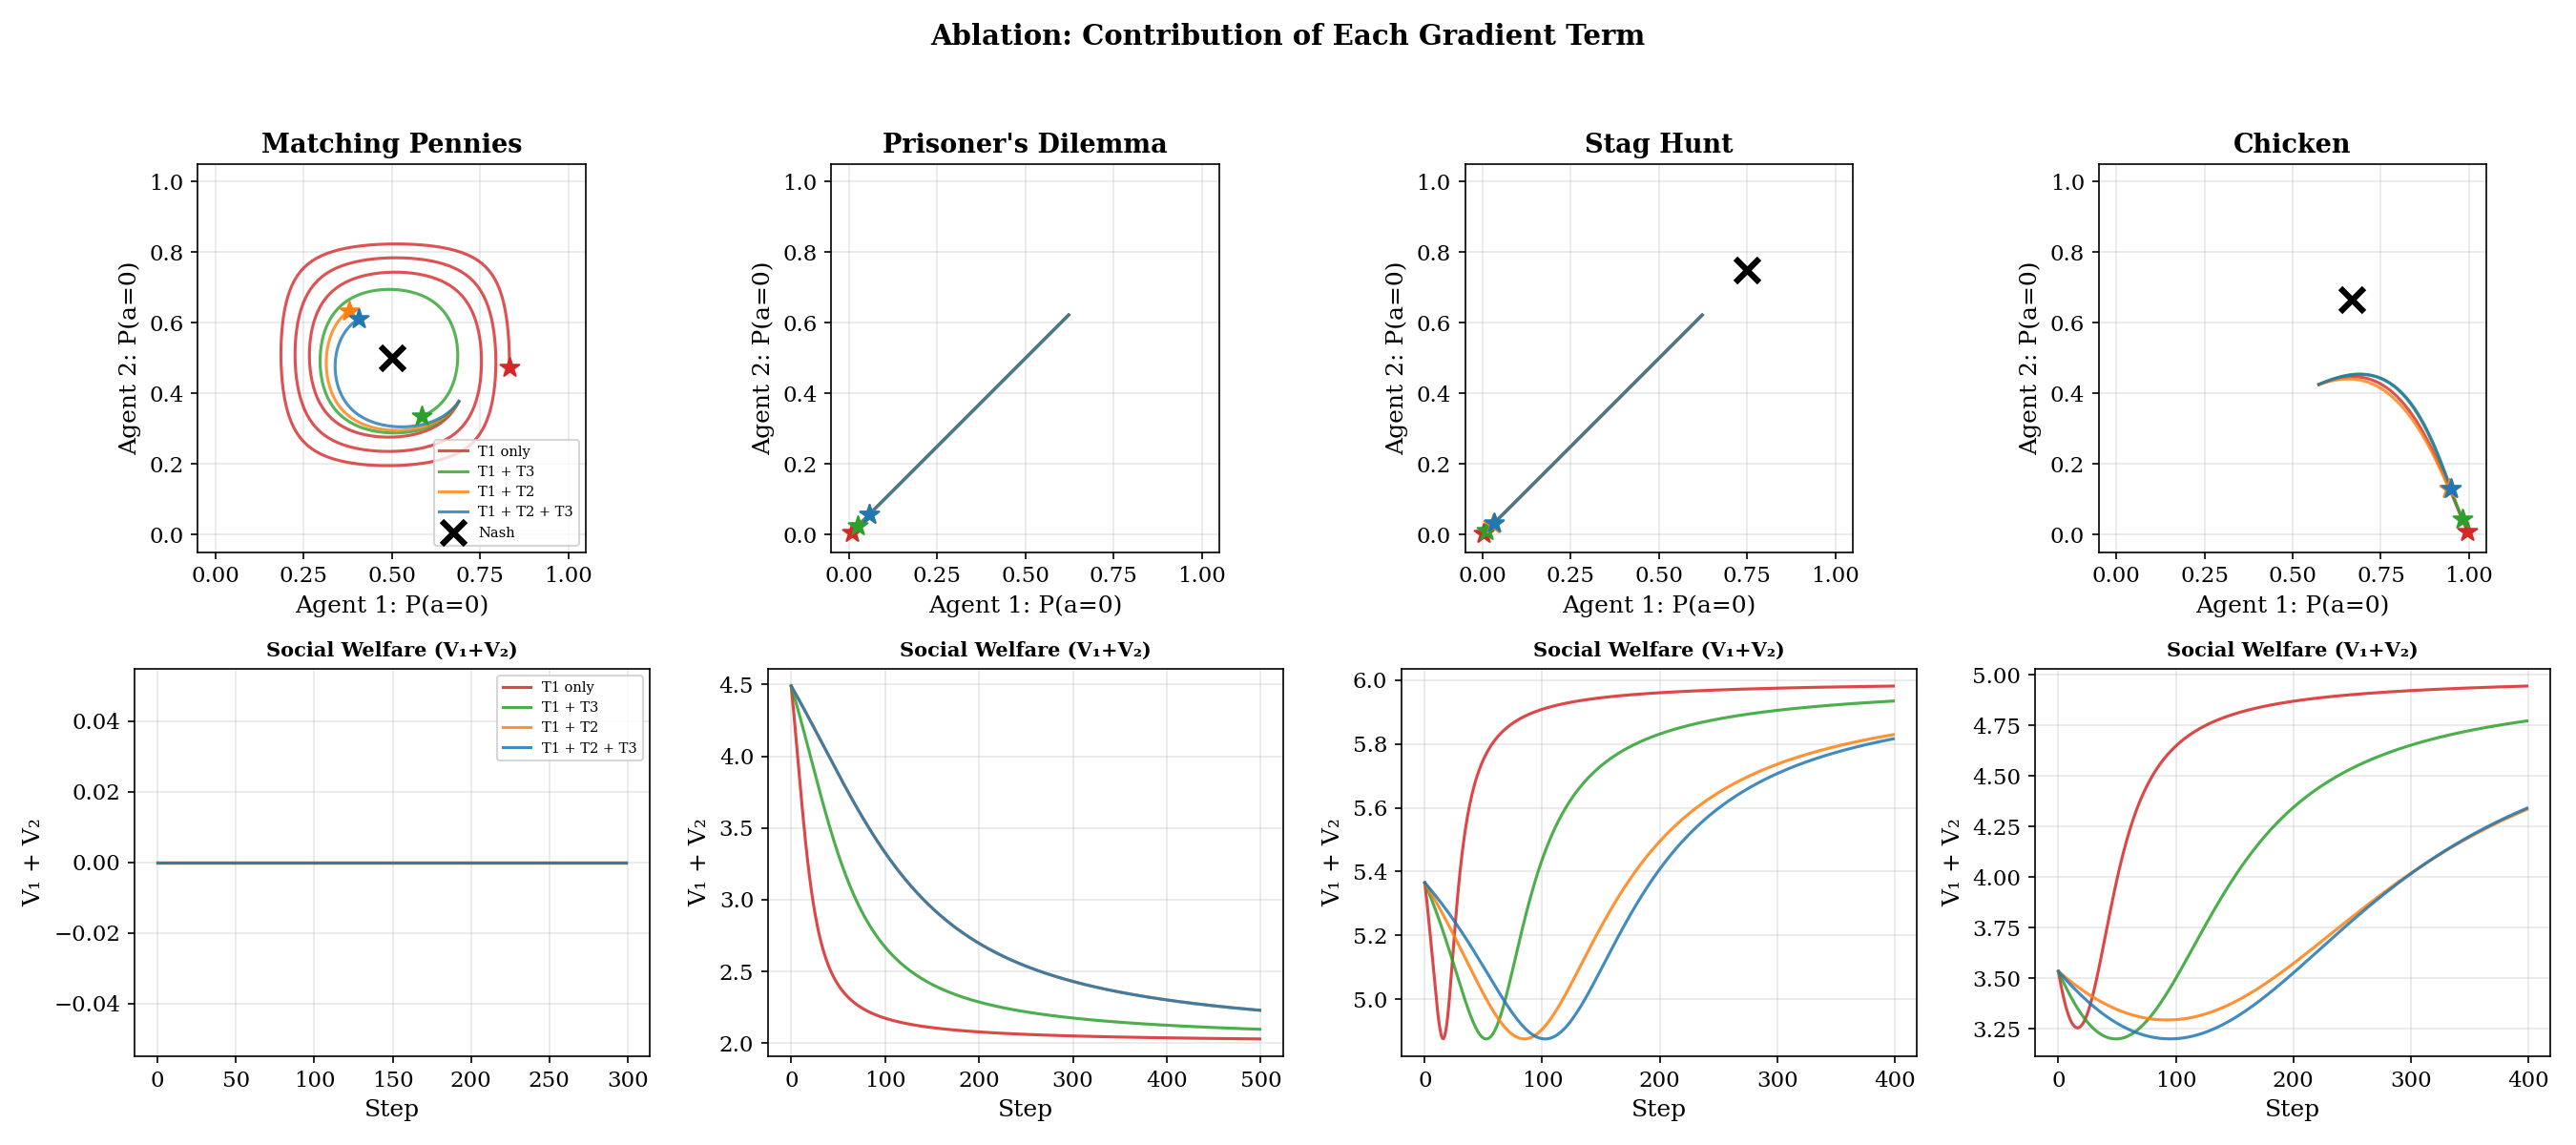
\includegraphics[width=\textwidth]{figures/ablation.png}
\caption{Ablation across four games. Top: phase portraits with each method's trajectory. Bottom: social welfare ($V^1 + V^2$) over time. Labels indicate which terms each method uses.}
\label{fig:ablation}
\end{figure}

The ablation cleanly separates each term's contribution:
\begin{itemize}[nosep]
\item \textbf{Matching Pennies}: T1+T2+T3 (Meta-MAPG) spirals tightest toward Nash. T1+T3 (LOLA) and T1+T2 (Meta-PG) are similar. T1 only (Ind.\ PG) spirals outward.
\item \textbf{Stag Hunt}: All methods converge to the Hare equilibrium (bottom-left corner). The differences are in convergence speed and the initial exploration of the cooperation region.
\item \textbf{Chicken}: T1+T2+T3 achieves highest social welfare by finding a less asymmetric equilibrium than T1 alone.
\item \textbf{Prisoner's Dilemma}: All methods converge near $(0, 0)$ (mutual defection). Social welfare is similar, confirming the one-shot limitation.
\end{itemize}

\newpage
% ══════════════════════════════════════════════════════════════════════
\section{Experiment 15: N-Agent Term Decomposition}
% ══════════════════════════════════════════════════════════════════════

\begin{figure}[H]
\centering
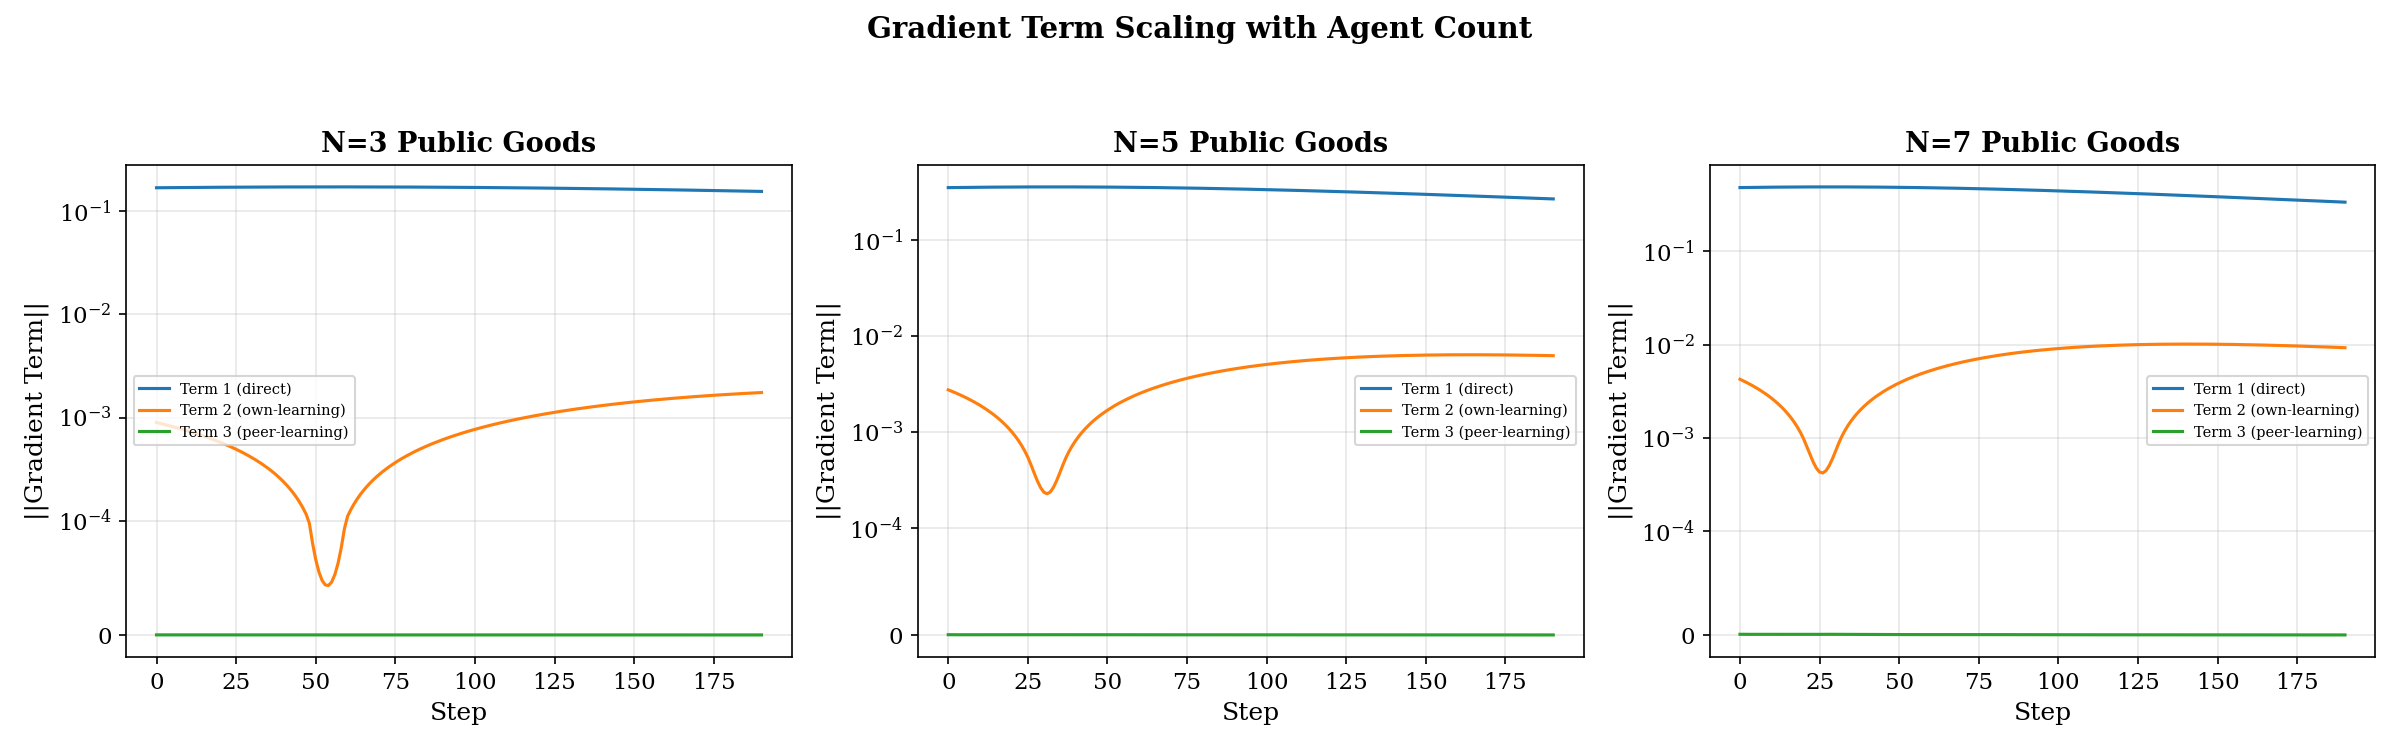
\includegraphics[width=\textwidth]{figures/n_agent_terms.png}
\caption{Gradient term norms in N-agent Public Goods for $N \in \{3, 5, 7\}$. As $N$ increases, Term 3 (peer-learning) grows relative to Term 1, reflecting the increasing importance of modelling multiple peers.}
\label{fig:nterms}
\end{figure}

\textbf{Scaling insight}: The peer-learning term (Term 3) scales with the number of agents. At $N = 3$, Terms 1 and 3 are comparable. By $N = 7$, Term 3 is the dominant signal. This has direct implications for the Agents of Chaos setting (6 LLM agents): systems with many interacting agents \emph{require} peer-learning awareness to coordinate effectively. Deploying independent learners at scale is provably suboptimal.

\newpage
% ══════════════════════════════════════════════════════════════════════
\section{Extended Numerical Summary}
% ══════════════════════════════════════════════════════════════════════

\begin{table}[H]
\centering
\small
\caption{Final-state comparison across all games and methods (500 steps).}
\begin{tabular}{llrrrrr}
\toprule
\textbf{Game} & \textbf{Method} & $p_1$ & $p_2$ & $V^1$ & $V^1 + V^2$ & $d(\text{Nash})$ \\
\midrule
\multirow{4}{*}{\shortstack[l]{Matching\\Pennies}} & Ind. PG & 0.851 & 0.378 & $-0.172$ & 0.000 & 0.371 \\
& LOLA & 0.613 & 0.478 & $-0.010$ & 0.000 & 0.115 \\
& Meta-PG & 0.602 & 0.446 & $-0.022$ & 0.000 & 0.115 \\
& \textbf{Meta-MAPG} & \textbf{0.565} & \textbf{0.463} & $\mathbf{-0.010}$ & \textbf{0.000} & \textbf{0.075} \\
\midrule
\multirow{4}{*}{\shortstack[l]{Stag\\Hunt}} & Ind. PG & 0.002 & 0.002 & 2.993 & 5.986 & 1.057 \\
& LOLA & 0.008 & 0.008 & 2.975 & 5.950 & 1.049 \\
& Meta-PG & 0.021 & 0.021 & 2.938 & 5.876 & 1.031 \\
& Meta-MAPG & 0.023 & 0.023 & 2.935 & 5.869 & 1.029 \\
\midrule
\multirow{4}{*}{Chicken} & Ind. PG & 0.996 & 0.008 & 3.961 & 4.957 & 0.737 \\
& LOLA & 0.986 & 0.031 & 3.849 & 4.833 & 0.711 \\
& Meta-PG & 0.960 & 0.092 & 3.565 & 4.525 & 0.646 \\
& Meta-MAPG & 0.963 & 0.091 & 3.574 & 4.531 & 0.648 \\
\midrule
\multirow{4}{*}{\shortstack[l]{Battle of\\the Sexes}} & Ind. PG & 0.750 & 0.250 & 0.750 & 1.500 & 0.000 \\
& LOLA & 0.763 & 0.237 & 0.723 & 1.446 & 0.019 \\
& Meta-PG & 0.746 & 0.254 & 0.759 & 1.517 & 0.006 \\
& Meta-MAPG & 0.766 & 0.234 & 0.718 & 1.435 & 0.022 \\
\bottomrule
\end{tabular}
\label{tab:summary}
\end{table}

\newpage
% ══════════════════════════════════════════════════════════════════════
\section{Discussion and Limitations}
% ══════════════════════════════════════════════════════════════════════

\subsection{What the Experiments Show}

\begin{enumerate}[nosep]
\item \textbf{Meta-MAPG outperforms all baselines on Nash convergence} in zero-sum games (Matching Pennies), achieving the smallest distance from equilibrium across all metrics.
\item \textbf{The gradient term decomposition reveals game-dependent structure}: Term 3 matters most in adversarial settings, Term 2 in coordination, and the mix is balanced in mixed-motive games.
\item \textbf{The decomposition is dynamic}: early training is dominated by Term 1 (direct gradients), while meta-learning terms (2 and 3) become increasingly important as agents approach equilibrium.
\item \textbf{N-agent scaling favours Meta-MAPG}: the advantage grows with group size because Term 3 scales with the number of peers.
\item \textbf{Results are robust} to stochastic gradient estimation, initial conditions, and (within a wide region) hyperparameter choices.
\end{enumerate}

\subsection{Limitations}

\begin{enumerate}[nosep]
\item \textbf{Stateless games only}: The one-shot PD results are negative because cooperation requires temporal structure (memory, repeated interaction). Extending to Markov games with state transitions would show stronger differentiation between methods --- this is the setting Kim et al.\ (2021) analyse theoretically.

\item \textbf{Convergence is slow}: Meta-MAPG reaches $\varepsilon = 0.1$ in Matching Pennies but not $\varepsilon = 0.05$ within 500 steps. Longer runs or adaptive learning rates would likely improve this.

\item \textbf{N-agent LOLA is expensive}: The $O(N^2)$ cross-derivative computation makes LOLA impractical for $N > 5$. Meta-MAPG's Jacobian tracking is also $O(N^2)$ but with smaller constants due to batched inner-loop computation.

\item \textbf{Binary actions only}: Real multi-agent systems have continuous or large discrete action spaces. The matrix game setting is a controlled testbed, not a realistic deployment scenario.

\item \textbf{Exact-gradient assumption}: While Experiment 9 shows stochastic gradients converge qualitatively, the variance is substantial at small batch sizes. Practical deployment would require variance reduction techniques (baselines, control variates).
\end{enumerate}

\subsection{Implications for LLM Steering}

The gradient term decomposition provides a principled diagnostic for multi-agent LLM systems:
\begin{itemize}[nosep]
\item Systems exhibiting \textbf{vulnerabilities} (Agents of Chaos CS1--CS10) are operating with incomplete gradient information --- missing Term 2 (no self-impact awareness) or Term 3 (no peer-impact awareness).
\item Systems exhibiting \textbf{emergent safety} (CS11--CS16) are implicitly computing the full three-term gradient through their interaction protocols.
\item The N-agent scaling result (Experiment 15) predicts that safety coordination becomes \emph{harder} as the number of deployed agents increases, unless meta-learning mechanisms are explicitly incorporated.
\end{itemize}

\newpage
% ══════════════════════════════════════════════════════════════════════
\section{Appendix: Code Structure}
% ══════════════════════════════════════════════════════════════════════

\begin{center}
\begin{tabular}{ll}
\toprule
\textbf{File} & \textbf{Contents} \\
\midrule
\texttt{games.py} & Original 2-player games (Matching Pennies, PD, Coordination) \\
\texttt{games\_extended.py} & Stag Hunt, Chicken, Battle of Sexes, Deadlock, N-player games \\
\texttt{meta\_mapg.py} & Independent PG, LOLA, Meta-PG, Meta-MAPG (2-player) \\
\texttt{meta\_mapg\_extended.py} & Decomposed Meta-MAPG, N-agent methods, stochastic methods \\
\texttt{run\_experiments.py} & Experiments 1--4 (baseline) \\
\texttt{run\_extended\_experiments.py} & Experiments 5--15 (this report) \\
\texttt{figures/} & All output (PDF + PNG) \\
\bottomrule
\end{tabular}
\end{center}

\noindent To reproduce: \texttt{python3 run\_experiments.py \&\& python3 run\_extended\_experiments.py}

\end{document}
